\documentclass[11pt]{article}
\usepackage[a4paper,margin=27mm,top=28mm,bottom=30mm]{geometry}
\usepackage[T1]{fontenc}
\usepackage[utf8]{inputenc}
\usepackage{mathpazo}
\usepackage[scaled=0.92]{helvet}
\usepackage{microtype}
\usepackage{amsmath,amssymb,amsthm,mathtools}
\usepackage{booktabs,array,tabularx}
\usepackage{enumitem}
\usepackage{tikz}
\usetikzlibrary{calc,arrows.meta}
\usepackage[colorlinks=true,linkcolor=black!70!blue,citecolor=black!60!blue,urlcolor=black!60!blue]{hyperref}
\usepackage[capitalise,noabbrev]{cleveref}
\usepackage{caption}
\captionsetup{font=small,labelfont=bf,width=0.92\textwidth}
\setlist{itemsep=2pt,topsep=3pt}
\linespread{1.04}
\theoremstyle{plain}
\newtheorem{theorem}{Theorem}[section]
\newtheorem{proposition}[theorem]{Proposition}
\newtheorem{lemma}[theorem]{Lemma}
\newtheorem{corollary}[theorem]{Corollary}
\theoremstyle{definition}
\newtheorem{definition}[theorem]{Definition}
\theoremstyle{remark}
\newtheorem{remark}[theorem]{Remark}
\newtheorem*{mainA}{Theorem A}
\newtheorem*{mainB}{Theorem B}
\newtheorem*{mainC}{Theorem C}
\newcommand{\Z}{\mathbb Z}
\newcommand{\N}{\mathbb N}
\newcommand{\Prob}{\mathbb P}
\newcommand{\Ex}{\mathbb E}
\newcommand{\eps}{\varepsilon}
\newcommand{\dtv}{d_{\mathrm{TV}}}
\newcommand{\ind}{\mathbf 1}
\newcommand{\Maj}{\operatorname{Maj}}
\newcommand{\Lh}[1]{\langle #1}
\newcommand{\Rh}[1]{#1\rangle}
\newcommand{\mA}{\mathsf A}
\newcommand{\mD}{\mathsf D}
\newcommand{\mC}{\mathsf C}
\newcommand{\blank}{\square}
\newcommand{\inv}{\dagger}
\newcommand{\act}{\mathrm{act}}
\newcommand{\frz}{\mathrm{frz}}
\newcommand{\col}{\operatorname{col}}
\newcommand{\nxt}{\operatorname{next}}
\newcommand{\dec}{\operatorname{dec}}
\newcommand{\digit}{\operatorname{dig}}
\newcommand{\msg}{\operatorname{msg}}
\newcommand{\rem}{\operatorname{rem}}
\newcommand{\car}{\operatorname{car}}
\newcommand{\SigQ}{\Sigma_Q}
\newcommand{\Hs}{\mathcal H}
\newcommand{\Ks}{\mathcal K}
\newcommand{\Xs}{\mathcal X}
\newcommand{\cF}{\mathcal F}
\hypersetup{pdftitle={A perturbed cellular automaton with infinitely many ergodicity transitions},pdfauthor={Seth Douglas and Nidhal Mghirbi}}
\title{\vspace{-1.2cm}\LARGE A perturbed cellular automaton\\ with infinitely many ergodicity transitions}
\author{Seth Douglas \and Nidhal Mghirbi}
\date{\small Version 1.0.0, November 2026}
\begin{document}
\maketitle
\begin{abstract}
\noindent
Can the ergodicity of one cellular automaton under noise switch on and off infinitely often as the noise rate decreases? Marsan, Sablik and T\"orm\"a built a one-dimensional automaton that is ergodic at small and at large noise rates and not ergodic in between, and asked which sets of rates can occur. We give one cellular automaton on $\Z^4$, with one finite alphabet and one neighbourhood, whose perturbation by independent uniform replacement of the whole symbol at rate $\eps$ has infinitely many alternating windows: open intervals of rates, with rational endpoints computable from their index and decreasing to $0$, on which the perturbed automaton alternately has two translation-invariant stationary laws and has one stationary law that attracts every initial law. The rule is given in full, including its action on malformed configurations.

The construction starts from a one-dimensional automaton whose unique stationary law makes a display bit mostly $1$ at the rates $b/(kB^k)$ with $k$ odd and mostly $0$ with $k$ even. Seeds created by the noise start base-$B$ counters. A changed counter letter makes its anchored prefix decay. The head freezes a previously validated message bit; once the length-parity messages have settled, this is the parity of the counter's length before the failure. Heads write their bits on the display. Independent copies of this automaton gate Toom's north-east-centre majority rule in two further dimensions, which keeps memory when the gates are mostly open and forgets when they are mostly closed. Through the correspondence between probabilistic cellular automata and space--time Gibbs measures, one finite-range interaction on $\Z^5$ with energies $0$ and $1$ has infinitely many computable alternating intervals of inverse temperature, tending to infinity, with at least two and with exactly one translation-invariant Gibbs measure. All windows lie at astronomically small noise rates.
\end{abstract}
\begin{center}\small AI systems assisted with this work; see ``How this work was done.''\end{center}
{\small\tableofcontents}

\section{Introduction}\label{sec:intro}

A probabilistic cellular automaton updates every site of a lattice at once; each site draws its new state from a law that depends on the old states of its neighbours. A basic way to obtain one is to perturb a deterministic cellular automaton $F$: apply $F$, then, independently at every site, replace the whole symbol with probability $\eps$ by a uniformly random symbol. The perturbed automaton $F_\eps$ is \emph{ergodic} if it has a unique stationary law and the law at time $t$ converges to it from every initial law, so that the process forgets its start. Every perturbed automaton is ergodic at all rates close to $1$, by a percolation argument \cite{MST19,MST26}. Toom's north-east-centre majority rule on $\Z^2$ keeps memory of its initial configuration at all small rates \cite{Toom80}, and G\'acs built a one-dimensional automaton with the same property \cite{Gacs01}. In these examples memory is lost as $\eps$ grows.

Marsan, Sablik and T\"orm\"a constructed a one-dimensional automaton whose perturbation is ergodic at small rates, not ergodic at an intermediate rate, and ergodic again at rates close to $1$ \cite{MST26}. They asked which sets $\{\eps:F_\eps\text{ is ergodic}\}$ can occur, recorded that no other kind of ergodicity transition was known, and noted that they do not know how many transitions their automaton, or G\'acs's, realizes. We show that one automaton can have infinitely many.

\begin{mainA}
There are a cellular automaton $F$ on $\Z^4$ with a finite alphabet and a finite neighbourhood, given explicitly in \cref{sec:rule,sec:four}, and open intervals $I_1,J_1,I_2,J_2,\dots$ of noise rates, with rational endpoints computable from the index, such that every rate in $I_n$ exceeds every rate in $J_n$, every rate in $J_n$ exceeds every rate in $I_{n+1}$, and $\sup I_n\to0$. For every $\eps\in I_n$ the perturbation $F_\eps$ has at least two translation-invariant stationary laws. For every $\eps\in J_n$ it has exactly one stationary law, and the law at time $t$ converges to it from every initial law.
\end{mainA}

Between $I_n$ and $J_n$ the ergodicity of $F_\eps$ changes at least once, so the set of rates at which $F_\eps$ is ergodic has infinitely many boundary points, accumulating at $0$. We do not determine the behaviour between the windows. \Cref{thm:mainA} gives the proof, and \cref{sec:four} gives the rule.

The space--time histories of a positive-rate probabilistic cellular automaton on $\Z^d$ are Gibbs measures on $\Z^{d+1}$ for an explicit interaction \cite{GKLM89,LMS90}. For a deterministic rule perturbed by uniform replacement this interaction has energies $0$ and $1$, and inverse temperature plays the role of the noise rate.

\begin{mainB}
There are a translation-invariant finite-range interaction $\Phi$ on $\Z^5$ with a finite alphabet and local energies in $\{0,1\}$, and open intervals $A_1<B_1<A_2<B_2<\cdots$ of inverse temperatures, with rational endpoints computable from the index and tending to infinity, such that $\beta\Phi$ has at least two translation-invariant Gibbs measures for every $\beta\in A_n$ and exactly one translation-invariant Gibbs measure for every $\beta\in B_n$.
\end{mainB}

Here translation invariance refers to all translations of $\Z^5$, and the uniqueness on $B_n$ is uniqueness among translation-invariant Gibbs measures; we do not know whether $\beta\Phi$ has Gibbs measures that are not translation invariant for $\beta\in B_n$. \Cref{thm:mainB} gives the proof.

\subsection{How the construction works}

The core is a one-dimensional automaton $Q$ with a binary \emph{display} coordinate $Y$.

\begin{mainC}
There are a cellular automaton $Q$ on $\Z$, given explicitly in \cref{sec:rule}, with a binary coordinate $Y$, and a rate $\eps_0>0$ such that for every $\eps\in(0,\eps_0)$ the perturbation $Q_\eps$ is ergodic, with stationary law $\pi_\eps$. With $\theta=1/(2^{32}3^8)$, $b=2^{70}$, $B=b^2$ and $\eps_k=b/(kB^k)$,
\begin{align*}
\pi_{\eps_k}\{Y(0)=1\}&>1-\theta&&\text{for every sufficiently large odd }k,\\
\pi_{\eps_k}\{Y(0)=1\}&<\theta&&\text{for every sufficiently large even }k.
\end{align*}
\end{mainC}

This is \cref{thm:source-ergodic,thm:oscillation}. In $Q$, rare \emph{seeds} appear only through the noise. A seed starts a \emph{head}, which moves at a fixed large speed, and next to it an anchored base-$B$ counter, which moves with the head and counts the age of the seed. The blocks of the counter pass the parity of its length towards the anchor as message bits, and the head copies the message bit of the anchor. The counter is built so that a single wrong symbol cannot be read as a different valid counter: a changed counter letter makes the anchored prefix that ends at the error erase itself, starting from the error and ending at the anchor. When the anchor disappears the head \emph{freezes} the bit it carries and keeps it for the rest of its life. So the head freezes a previously validated message bit; once the length-parity messages have settled, this is the parity of the counter's length before the failure. As it moves, the head writes its bit on the display bits that it passes, and the display keeps the last value written. At the rate $\eps_k$, the first error in a counter of a typical seed occurs while the counter has length $k$ and its messages have settled, so most frozen heads, and hence most display bits, carry the parity of $k$. A \emph{sweeper} emitted by each seed clears the space in front of its counter, so that material left in the configuration from earlier times cannot interfere, and a family of independent \emph{erasers} cuts every long chain of dependence in the counters, which makes $Q_\eps$ forget its initial configuration at every positive rate below $\eps_0$.

The automaton $F$ of Theorem~A runs independent copies of $Q$ along one coordinate of $\Z^4$, which move one step per update in a second coordinate, and uses their display bits as gates for north-east-centre majority on bits in the remaining two coordinates. In a fixed plane the gates are then independent, as in \cite{DMnil}, and a gate is open with probability $\pi_\eps\{Y(0)=1\}$. When the gates are mostly open, Toom's stability theorem, in the quantitative form of G\'acs \cite{Gacs21}, preserves two phases; when they are mostly closed, dependence on the initial bits dies out. A dovetailed search over finite-time certificates turns the oscillation of Theorem~C into computable intervals. \Cref{fig:mechanism} sketches both levels.

\begin{figure}[t]
\centering
\resizebox{\textwidth}{!}{%
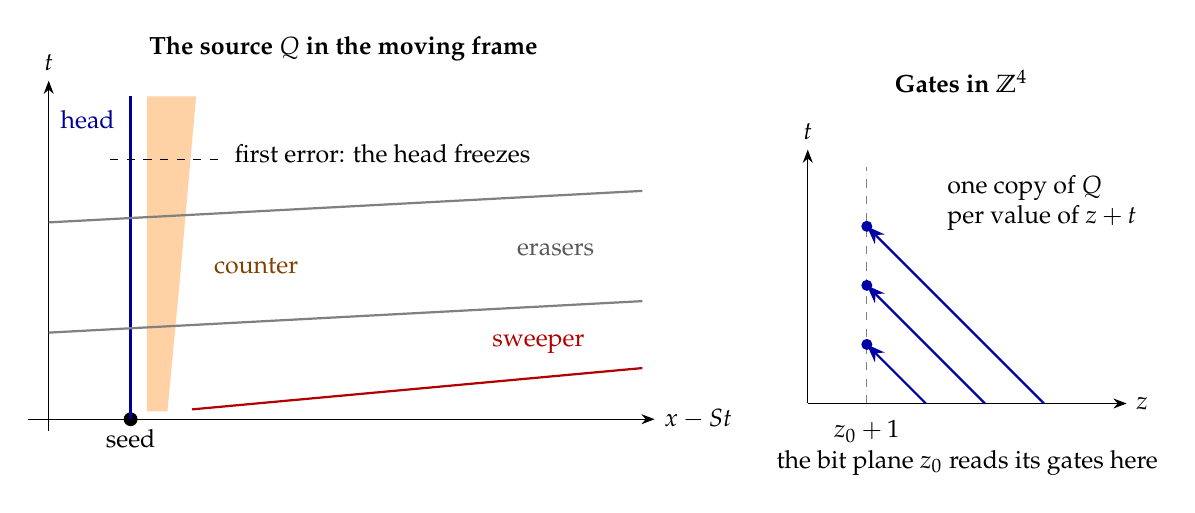
\begin{tikzpicture}[font=\small,>=Stealth]
\begin{scope}[x=0.52cm,y=0.5cm]
\node[font=\small\bfseries] at (5.2,9.4) {The source $Q$ in the moving frame};
\draw[->] (-2.5,0)--(12.8,0) node[right] {$x-St$};
\draw[->] (-2,-0.3)--(-2,8.6) node[above] {$t$};
\fill (0,0) circle (2.5pt) node[below] {seed};
\draw[very thick,blue!60!black] (0,0)--(0,8.2);
\node[blue!60!black,anchor=east] at (-0.15,7.6) {head};
\fill[orange!35] (0.4,0.2)--(0.4,8.2)--(1.6,8.2)--(1.2,3.5)--(0.9,0.2)--cycle;
\node[orange!50!black,anchor=west] at (1.8,3.9) {counter};
\draw[thick,red!70!black] (1.5,0.25)--(12.5,1.3);
\node[red!70!black,anchor=west] at (8.6,1.9) {sweeper};
\draw[thick,gray] (-2,2.2)--(12.5,3.0);
\draw[thick,gray] (-2,5.0)--(12.5,5.8);
\node[gray!70!black,anchor=west] at (9.2,4.3) {erasers};
\draw[dashed] (-0.5,6.6)--(2.2,6.6);
\node[anchor=west] at (2.3,6.75) {first error: the head freezes};
\end{scope}
\begin{scope}[shift={(8.6,0.2)},x=0.75cm,y=0.75cm]
\node[font=\small\bfseries] at (2.6,5.45) {Gates in $\Z^4$};
\draw[->] (0,0)--(5.4,0) node[right] {$z$};
\draw[->] (0,0)--(0,4.3) node[above] {$t$};
\draw[dashed,gray] (1,0)--(1,4);
\foreach \k in {1,2,3} {
\draw[blue!65!black,thick,->] (1+\k,0)--(1,\k);
\fill[blue!65!black] (1,\k) circle (2pt);
}
\node[anchor=west,align=left] at (2.2,3.4) {one copy of $Q$\\ per value of $z+t$};
\node[anchor=north] at (1,-0.12) {$z_0+1$};
\node[align=center] at (2.7,-1.0) {the bit plane $z_0$ reads its gates here};
\end{scope}
\end{tikzpicture}}
\caption{Left: in coordinates moving with the heads, a seed starts a head, a counter that grows slowly to its right, and a sweeper that clears the region in front of the counter; erasers move to the right through everything. Not to scale. Right: the copies of $Q$ move down in $z$ by one step per update, so the gates read by a fixed bit plane at successive times come from different, independent copies.}
\label{fig:mechanism}
\end{figure}

\subsection{What the theorems do not say}

\paragraph{Dimension.} The source $Q$ is one-dimensional. Two more dimensions carry Toom's rule and one more makes the gates independent. The question of Marsan, Sablik and T\"orm\"a in dimension one, where non-ergodicity is much harder to obtain, remains open, and we do not address dimensions two and three.

\paragraph{Scale.} The alphabet of $F$ has more than $3^{3^{9216}}$ symbols, and the rates involved are astronomically small. Our estimates say nothing about indices $k$ up to the number $3^{9216}$ of eraser tracks, so the windows they guarantee lie at rates below $2^{-140\cdot3^{9216}}$. The windows are defined by a terminating search; we have not located any of them.

\paragraph{Nilpotency.} The automaton $F$ is not nilpotent (\cref{rem:not-nilpotent}). In \cite{DMnil} we built, for every $n$, a nilpotent automaton with $n$ windows; whether one nilpotent automaton can have infinitely many remains open.

\paragraph{Gibbs measures.} Theorem~B concerns translation-invariant Gibbs measures only.

\subsection{Prior work}

\Cref{tab:landscape} lists the closest results. Marsan and Sablik showed that for continuous maps of $A^{\N}$ that need not commute with the shift, the set of rates with a unique stationary law can be any $G_\delta$ subset of $[0,1]$ containing $1$, and that for cellular automata the possible sets are not characterized \cite{MS25}. In an earlier paper they showed that the stationary laws of a perturbed one-dimensional cellular automaton can oscillate as $\eps\to0$, realizing every $\Pi_2$-computable connected compact set of measures as the set of zero-noise limits \cite{MS24}; their construction also starts computations from symbols that only the noise creates, and gives younger computations priority. For one fixed lattice model, infinite sequences of phase transitions in temperature are known for continuous spins: van Enter and Ruszel describe a nearest-neighbour model of circle-valued spins with nested potential wells which, in dimension at least two, has an infinite sequence of first-order transitions alternating between ferromagnetic and antiferromagnetic order \cite[Section~2]{vER07}, and they attribute this to van Enter and Shlosman \cite{vES05}; Byington and Socolar report an infinite sequence of freezing transitions in a two-dimensional model with a limit-periodic ground state \cite{BS12}. Gibbs measures of finite-range models with a finite alphabet need not converge as the temperature tends to zero \cite{CH10,GST}. In \cite{DMhard} we gave one nearest-neighbour interaction on $\Z^2$ with energies $0$, $1$ and $+\infty$ and explicit intervals $J_n$ of inverse temperature on which it has exactly one translation-invariant Gibbs measure if a fixed universal machine does not halt on input $n$, and at least two if it halts; that model has infinitely many intervals of each kind, but which intervals are of which kind is undecidable, and its hard constraints are essential. The interaction of Theorem~B has finite energies, every local pattern has positive weight, and both kinds of intervals are computable; it lives in dimension five. Toom's rule has also been used to stabilize computation inside Gibbs measures of finite-range models \cite{MT25}.

\begin{table}[t]
\centering\small
\begin{tabularx}{\textwidth}{@{}>{\raggedright\arraybackslash}p{0.25\textwidth} >{\raggedright\arraybackslash}X >{\raggedright\arraybackslash}p{0.22\textwidth}@{}}
\toprule
Result & Statement & Alternations\\
\midrule
Marsan--Sablik--T\"orm\"a \cite{MST26} & One-dimensional automaton: ergodic, not ergodic, ergodic as the rate increases. & At least two transitions; total unknown\\[4pt]
Marsan--Sablik \cite{MS25} & Continuous maps of $A^{\N}$, not cellular automata: every $G_\delta$ set containing $1$ is a set of rates with a unique stationary law. & Arbitrary\\[4pt]
Douglas--Mghirbi \cite{DMnil} & For every $n$, a nilpotent automaton on $\Z^3$ with $n$ windows of two stationary laws between windows of ergodicity. & At least $2n$ transitions; the rule depends on $n$\\[4pt]
van Enter--Ruszel \cite{vER07} & Circle-valued spins, nearest neighbour, nested wells: first-order transitions accumulating at zero temperature \cite[Section~2]{vER07}, attributed there to van Enter--Shlosman \cite{vES05}. & Infinitely many\\[4pt]
Douglas--Mghirbi \cite{DMhard} & Interaction on $\Z^2$ with energies $0,1,+\infty$; translation-invariant uniqueness on $J_n$ if and only if a universal machine does not halt on $n$. & Infinitely many; undecidable which\\[4pt]
Theorem~A & Automaton on $\Z^4$: windows of two stationary laws alternating with windows of ergodicity. & Infinitely many, computable\\[4pt]
Theorem~B & Interaction on $\Z^5$ with energies $0,1$: windows of translation-invariant non-uniqueness and uniqueness. & Infinitely many, computable\\
\bottomrule
\end{tabularx}
\caption{Related phase-diagram results. ``Windows'' are open intervals of the parameter.}
\label{tab:landscape}
\end{table}

\paragraph{Reading guide.} \Cref{sec:setting} fixes definitions, proves a coupling criterion for ergodicity, and states Toom's stability theorem in G\'acs's form. \Cref{sec:rule} defines the source automaton $Q$ completely, field by field, including its action on malformed configurations; a reader who wants to implement it needs only this section. \Cref{sec:source-ergodic} proves that $Q_\eps$ forgets its initial configuration at every rate in $(0,\eps_0)$. \Cref{sec:counter} studies the counter, and \cref{sec:display} proves the oscillation of Theorem~C. \Cref{sec:four} builds the four-dimensional automaton and proves Theorem~A, and \cref{sec:gibbs} deduces Theorem~B. A reader interested only in the four-dimensional step can take Theorem~C as given and read \cref{sec:setting,sec:four}.

\section{Setting}\label{sec:setting}

\subsection{Perturbed cellular automata}

Write $\N=\{0,1,2,\dots\}$. Let $\Sigma$ be a finite alphabet and $d\ge1$. A \emph{cellular automaton} on $\Sigma^{\Z^d}$ is given by a finite neighbourhood $N\subset\Z^d$ and a local rule $f\colon\Sigma^N\to\Sigma$, and maps a configuration $x$ to $(Fx)(v)=f\bigl((x(v+n))_{n\in N}\bigr)$. For $0<\eps<1$, its \emph{perturbation by uniform replacement at rate $\eps$}, written $F_\eps$, is the following Markov process. At every site $v$ and time $t\ge1$ there are a \emph{flag} $R_t(v)\in\{0,1\}$ with $\Prob(R_t(v)=1)=\eps$ and a \emph{mark} $U_t(v)$, uniform on $\Sigma$, all independent. The state at time $t$ is
\[
X_t(v)=\begin{cases}U_t(v),&R_t(v)=1,\\ (FX_{t-1})(v),&R_t(v)=0.\end{cases}
\]
We call the family of flags and marks the \emph{noise}. Given $X_{t-1}$, the new symbols are independent over sites, and the new symbol at $v$ equals $s$ with probability $(1-\eps)\ind\{s=(FX_{t-1})(v)\}+\eps/|\Sigma|$. Every such probability is positive, so $F_\eps$ is a probabilistic cellular automaton with positive rates.

A \emph{stationary law} is a probability measure $\mu$ on $\Sigma^{\Z^d}$, with the product topology, such that $X_0\sim\mu$ implies $X_1\sim\mu$. It is \emph{translation invariant} if it is invariant under the translations of $\Z^d$. The perturbation $F_\eps$ is \emph{ergodic} if it has exactly one stationary law $\mu$ and the law of $X_t$ converges weakly to $\mu$ from every initial law. The configuration space is compact and a local observable after one update depends continuously on finitely many old symbols, so every weak limit point of the Ces\`aro averages $T^{-1}\sum_{t<T}\mathrm{Law}(X_t)$ is a stationary law. In particular a stationary law exists.

\subsection{A coupling criterion}

Run all initial configurations with the same noise, and write $X_t^x$ for the configuration at time $t$ started from $X_0=x$. For a finite set $O\subset\Z^d$ and $t\ge0$, the event
\[
\mathcal C(O,t)=\bigl\{X^x_t|_O=X^y_t|_O\ \text{for all configurations }x,y\bigr\}
\]
says that the time-$t$ symbols on $O$ do not depend on the initial configuration. These symbols depend on the initial configuration and the noise only through a finite space--time region, so $\mathcal C(O,t)$ is determined by finitely many noise variables. We say that $F_\eps$ \emph{coalesces} if $\Prob(\mathcal C(O,t))\to1$ as $t\to\infty$ for every finite $O$.

\begin{lemma}\label{lem:coalesce}
Suppose that $F_\eps$ coalesces. Then $F_\eps$ has exactly one stationary law $\pi$, and $\pi$ is translation invariant. For every initial law $\nu$, every finite $O$ and every $t$, the law $\nu_t$ of $X_t$ satisfies $\dtv\bigl((\nu_t)_O,\pi_O\bigr)\le1-\Prob(\mathcal C(O,t))$. In particular $F_\eps$ is ergodic.
\end{lemma}

\begin{proof}
Let $\nu,\nu'$ be initial laws and draw $X_0\sim\nu$, $X_0'\sim\nu'$ independently of the noise. On $\mathcal C(O,t)$ the two runs agree on $O$ at time $t$, so the total variation distance between their laws on $O$ is at most $1-\Prob(\mathcal C(O,t))$. Taking $\nu'$ stationary gives the bound; two stationary laws then have the same marginal on every finite set, so they are equal. A translate of $\pi$ is stationary, because $F_\eps$ commutes with translations, so it equals $\pi$.
\end{proof}

When $F_\eps$ coalesces, its stationary law is a function of the past noise. Index the noise by all times $t\in\Z$.

\begin{lemma}[Stationary history]\label{lem:history}
Suppose that $F_\eps$ coalesces. There is a process $(X_t)_{t\in\Z}$ such that each $X_t$ is a measurable function of the noise at times at most $t$, each $X_t$ has law $\pi$, and for every $t$ the configuration $X_t$ is obtained from $X_{t-1}$ and the noise at time $t$ by the update rule.
\end{lemma}

\begin{proof}
For $s<t$ and finite $O$, let $\mathcal C_{s,t}(O)$ be the event that the symbols on $O$ at time $t$, for runs started at time $s$, do not depend on the configuration at time $s$. These events increase as $s$ decreases, since a constant map stays constant when composed with an earlier map, and $\Prob(\mathcal C_{s,t}(O))=\Prob(\mathcal C(O,t-s))\to1$. So almost surely the common value on $O$ is the same for all $s$ below some finite random time; call it $X_t|_O$. These values are consistent in $O$, satisfy the update rule, and are functions of the noise at times at most $t$. Started from a fixed configuration at time $s$, the law on $O$ at time $t$ differs from that of $X_t|_O$ by at most $1-\Prob(\mathcal C(O,t-s))$, and by \cref{lem:coalesce} it converges to $\pi_O$; hence $X_t\sim\pi$.
\end{proof}

We call $(X_t)_{t\in\Z}$ the \emph{stationary history}. Its law is invariant under all space--time translations, because the law of the noise is. We write $\cF_t$ for the $\sigma$-field generated by the noise at times at most $t$; then $X_t$ is $\cF_t$-measurable and the noise at time $t+1$ is independent of $\cF_t$.

\subsection{Toom's stability theorem}

We use the explicit infinite-plane estimate in G\'acs's exposition \cite{Gacs21} of the Berman--Simon proof \cite{BermanSimon88} of Toom's theorem \cite{Toom80}. Write $\mathbf e_1,\mathbf e_2$ for the unit vectors of $\Z^2$ and $\Maj$ for the majority of three bits.

\begin{theorem}[Toom stability, quantitative specialization]\label{thm:toom}
Let a binary process $(\xi_t)_{t\ge0}$ on $\Z^2$, started from the constant configuration $a\in\{0,1\}$, be a $\gamma$-perturbation of north-east-centre majority: conditional on the past and on the other updates at the same time, each site update $\xi_{t+1}(p)$ disagrees with $\Maj(\xi_t(p),\xi_t(p+\mathbf e_1),\xi_t(p+\mathbf e_2))$ with probability at most $\gamma$. If
\begin{equation}\label{eq:tau}
\gamma<\tau:=\frac1{32\cdot24^8}=\frac1{2^{29}3^8},
\end{equation}
then at every site and time the probability that $\xi_t(p)\ne a$ is at most $96\gamma$.
\end{theorem}

This is the case $m=\infty$ of \cite[Theorem~1.6]{Gacs21},\footnote{In the displayed perturbation condition of \cite[Definition~1.3]{Gacs21}, the comparison with the prescribed output is printed as equality. We use the disagreement event specified by its subsequent definition of $\mathrm{Noise}$ (Definition~1.7) and its proof.} specialized as follows. Take the auxiliary one-dimensional space of its Definition~1.5 to be a singleton and its transition rule the identity; the rule is then north-east-centre majority on the remaining two coordinates. The reference trajectory is $a$ at every site and time. The constants stated there are $r=24$, threshold $(32r^8)^{-1}$ and error bound $4r\gamma$. We apply it to processes of the following form. Each site's update is determined by the plane's past and fresh local randomness independent across sites and times. It obeys majority unless a local event of probability at most $\gamma$ occurs. Such a process is a $\gamma$-perturbation. Toom's theorem itself, with an unspecified threshold, is \cite{Toom80}.

\section{The source automaton}\label{sec:rule}

This section defines the one-dimensional automaton $Q$ of Theorem~C completely. Every symbol of the alphabet and every local configuration, including malformed ones, has a specified image.

\subsection{Constants}

The constants are fixed in \cref{tab:constants}. Each is defined by a formula or by a terminating search over integers with exact rational comparisons, and the values shown follow from the definitions by direct arithmetic. For $b$: with $b=2^c$ the condition reads $2^{5-c}+2^{-2^{c-6}}<2^{-43}3^{-10}7^{-2}$, and $3^{10}7^2=2893401$ lies between $2^{21}$ and $2^{22}$, so $c=70$ satisfies it and $c=69$ does not. For $S$: $16\Lambda/\theta=2^4\cdot(2^33^27^2)\cdot2^{32}3^8$ is already an even integer. Two relations will be used repeatedly:
\begin{equation}\label{eq:constant-relations}
\Lambda/S=\theta/16,\qquad 2^{-n_0}\le\theta/8 .
\end{equation}

\begin{table}[ht]
\centering\small
\begin{tabularx}{\textwidth}{@{}l >{\raggedright\arraybackslash}X >{\raggedright\arraybackslash}p{0.24\textwidth}@{}}
\toprule
Symbol & Definition and value & Role\\
\midrule
$\tau$ & $1/(32\cdot24^8)=2^{-29}3^{-8}$ & Toom threshold\\
$\theta$ & $\tau/8=2^{-32}3^{-8}$ & display error at $\eps_k$\\
$\Lambda$ & $72(n_0+1)$, with $n_0$ least such that $2^{-n_0}\le\theta/8$; so $n_0=48$ and $\Lambda=3528$ & display lookback\\
$S$ & least even integer $\ge16\Lambda/\theta$; so $S=2^{39}3^{10}7^2\approx1.59\cdot10^{18}$ & speed of moving fields\\
$\delta$ & $\theta/(32\Lambda)=2^{-40}3^{-10}7^{-2}$ & fraction of wrong heads\\
$b$ & least power of two $\ge64$ with $32/b+2^{-\lfloor b/64\rfloor}<\delta/8$; so $b=2^{70}$ & \\
$B$ & $b^2=2^{140}$ & counter base\\
$N_{\mathrm s}$ & least integer $\ge9$ with $4/(N_{\mathrm s}^2+4)<\delta/8$, that is, with $N_{\mathrm s}^2>2^{45}3^{10}7^2-4$; so $N_{\mathrm s}\approx1.009\cdot10^{10}$ & seed letters per side\\
$\ell$ & $1152$ & eraser block parameter\\
$M$ & $3^{8\ell}=3^{9216}$ & number of eraser tracks\\
$\eps_0$ & $1/(2\ell)=1/2304$ & range of rates\\
\bottomrule
\end{tabularx}
\caption{The constants of the source automaton $Q$.}
\label{tab:constants}
\end{table}

\subsection{The alphabet}

Several fields of $Q$ carry \emph{blocks}. In such a field a letter is $0$ or a \emph{half}: a left half $\Lh y$ or a right half $\Rh y$, with a \emph{payload} $y$ from a set fixed for the field. A \emph{block at $a$} with payload $y$ is the left half $\Lh y$ at site $a$ followed by the right half $\Rh y$ at site $a+1$, with the same payload; $a$ is its \emph{anchor}. Two blocks never overlap, because the site $a+1$ of a block carries a right half and cannot be the left site of another block. When the payload set has one element we write the halves as $\langle$ and $\rangle$ and call a block a \emph{pair}.

A symbol of $Q$ has the following five fields.
\begin{enumerate}[label=(\arabic*)]
\item \emph{Eraser tracks} $E_1,\dots,E_M$, each with letters $0,\langle,\rangle$.
\item A \emph{sweeper track} $W$ with letters $0,\langle,\rangle$.
\item A \emph{head field} $H$ with the letter $0$; \emph{seed letters} $\sigma_u$ and $\sigma'_u$ for $1\le u\le N_{\mathrm s}$; and halves $\Lh q,\Rh q$ for the four \emph{head states}
\[
q\in\{\act_0,\act_1,\frz_0,\frz_1\}.
\]
The \emph{left-type} letters are the $\sigma_u$ and the $\Lh q$, the \emph{right-type} letters the $\sigma'_u$ and the $\Rh q$. The field has $|\Hs|=2N_{\mathrm s}+9$ letters.
\item A \emph{counter field} $K$ with the letter $0$ and halves $\Lh y,\Rh y$ whose payloads $y$ are the \emph{macrostates}
\[
\mA_{d,m},\ \mD_{d,m}\quad(0\le d\le B,\ m\in\{0,1\}),\qquad \mC_c\quad(c\in\{0,1\}).
\]
We call them \emph{anchor digits}, \emph{digits} and \emph{caps}; $d$ is the \emph{digit value}, $m$ and $c$ are the \emph{message bits}. Write $\Xs$ for the set of macrostates; $|\Xs|=4B+6$, and the field has $|\Ks|=8B+13$ letters.
\item A \emph{display bit} $Y\in\{0,1\}$.
\end{enumerate}
The alphabet of $Q$ is $\SigQ=\{0,\langle,\rangle\}^M\times\{0,\langle,\rangle\}\times\Hs\times\Ks\times\{0,1\}$, of size $2\cdot3^{M+1}(2N_{\mathrm s}+9)(8B+13)$. A uniform symbol of $\SigQ$ has independent uniform fields.

\subsection{Patterns read by the rule}

Fix an old row $x\in\SigQ^\Z$ and write $E_m(a),W(a),H(a),K(a),Y(a)$ for the fields of $x(a)$.

\begin{definition}[Patterns]\label{def:patterns}
\begin{enumerate}[label=(\alph*)]
\item An \emph{eraser pair of track $m$ at $a$} means $E_m(a)=\langle$ and $E_m(a+1)=\rangle$. A \emph{sweeper pair at $a$} means $W(a)=\langle$ and $W(a+1)=\rangle$.
\item A \emph{raw seed at $a$} means $H(a)=\sigma_u$ and $H(a+1)=\sigma'_v$ for some $u,v$. It is \emph{accepted} if there is no raw seed at any $a'$ with $1\le|a'-a|\le512$. Distinct accepted seeds are more than $512$ apart.
\item A \emph{head at $a$} is a raw seed at $a$, or $H(a)=\Lh q$ and $H(a+1)=\Rh q$ with the same state $q$. Two heads never overlap, since $H(a)$ is of left type and $H(a+1)$ of right type. The \emph{colour} of a head is $1$ for a raw seed and $c$ for the states $\act_c$ and $\frz_c$.
\item The \emph{next state} of a head at $a$ is
\[
\nxt(a)=\begin{cases}
\act_1,&\text{raw seed at }a,\\
\frz_c,&H(a)=\Lh{\frz_c},\\
\act_m,&H(a)=\Lh{\act_c}\text{ and a block with payload }\mA_{d,m}\text{ is at }a+2,\\
\frz_c,&H(a)=\Lh{\act_c}\text{ otherwise}.
\end{cases}
\]
\end{enumerate}
\end{definition}

So an active head reads the block two sites to its right. If it is an anchor digit, the head copies its message bit; otherwise the head freezes with its current colour. A frozen head never changes.

\subsection{The counter's macro rule}\label{subsec:macro}

The counter field is read in blocks. For an integer $a$ put
\[
\dec(a)=\begin{cases}\blank,&K(a)=K(a+1)=0,\\ y,&\text{a block with payload }y\text{ is at }a,\\ \inv,&\text{otherwise,}\end{cases}
\]
the \emph{macrocell} at $a$; $\blank$ is an empty macrocell and $\inv$ an invalid one. For a digit value $d$ put $\rem(d)=d$ if $d<B$, $\rem(B)=0$, and $\car(d)=\ind\{d=B\}$. Put $\digit(\mA_{d,m})=\digit(\mD_{d,m})=d$, $\msg(\mA_{d,m})=\msg(\mD_{d,m})=m$ and $\msg(\mC_c)=c$. Write $\mathfrak A$, $\mathfrak D$, $\mathfrak C$ for the sets of anchor digits, digits and caps.

\begin{definition}[Macro rule]\label{def:macro}
Let a block with payload $y$ be at $a$, and put $\lambda=\dec(a-2)$, $\rho=\dec(a+2)$ and $\rho'=\dec(a+4)$. Its \emph{new payload} $y'\in\Xs\cup\{\blank\}$ is given by \cref{tab:macro}. A site $t$ is a \emph{growth target} with payload $\mC_{1-c}$ if $\dec(t)=\blank$, a block with payload $\mC_c$ is at $t-2$, $\dec(t-4)\in\mathfrak A\cup\mathfrak D$ with $\digit(\dec(t-4))=B$, and $\dec(t+2)=\blank$. A test on a macrocell equal to $\inv$ always fails.
\end{definition}

\begin{table}[ht]
\centering\small
\begin{tabularx}{\textwidth}{@{}l >{\raggedright\arraybackslash}X l@{}}
\toprule
Old payload & Condition & New payload\\
\midrule
$\mA_{d,m}$ & $\rho\in\mathfrak D\cup\mathfrak C$ & $\mA_{\rem(d)+1,\,\msg(\rho)}$\\
 & otherwise & $\blank$\\[3pt]
$\mD_{d,m}$ & $\lambda\in\mathfrak A\cup\mathfrak D$ and $\rho\in\mathfrak D\cup\mathfrak C$ & $\mD_{\rem(d)+\car(\digit(\lambda)),\,\msg(\rho)}$\\
 & otherwise & $\blank$\\[3pt]
$\mC_c$ & $\lambda\in\mathfrak A\cup\mathfrak D$, $\digit(\lambda)<B$ and $\rho=\blank$ & $\mC_c$\\
 & $\lambda\in\mathfrak A\cup\mathfrak D$, $\digit(\lambda)=B$, $\rho=\blank$ and $\rho'=\blank$ & $\mD_{1,1-c}$\\
 & otherwise & $\blank$\\
\bottomrule
\end{tabularx}
\caption{The macro rule of the counter. An anchor digit reads only its right neighbour.}
\label{tab:macro}
\end{table}

All new digit values lie in $\{0,\dots,B\}$. A cap whose left neighbour has digit value $B$ becomes a digit exactly when the empty macrocell to its right is a growth target, since both conditions test the same three macrocells. So a counter either grows by one block or loses its cap; a failed growth never leaves a shorter valid counter.

\begin{definition}[Counter proposal]\label{def:compiled}
For $x\in\Z$, the \emph{counter proposal} $\kappa(x)\in\Ks$ is
\[
\kappa(x)=\begin{cases}
\Lh{y'},&\text{a block is at }x\text{ and its new payload is }y'\ne\blank,\\
\Rh{y'},&\text{a block is at }x-1\text{ and its new payload is }y'\ne\blank,\\
\Lh{\mC_{1-c}},&x\text{ is a growth target with payload }\mC_{1-c},\\
\Rh{\mC_{1-c}},&x-1\text{ is a growth target with payload }\mC_{1-c},\\
0,&\text{otherwise.}
\end{cases}
\]
\end{definition}

The four cases exclude each other: a block at $x$ makes $K(x)$ a left half, a block at $x-1$ makes it a right half, and a growth target at $x$ or at $x-1$ requires $K(x)=0$; growth targets at both $x-1$ and $x$ would require $K(x-1)=0$ and a block at $x-2$, whose right half is $K(x-1)$. The proposal $\kappa(x)$ depends only on $K(x-5),\dots,K(x+5)$.

\subsection{The rule}

\begin{definition}[The source automaton $Q$]\label{def:Q}
Let $x$ be the old row. The new symbol at a site $i$ is computed as follows, with $j=i-S$.
\begin{enumerate}[label=(\arabic*)]
\item \emph{Erasers.} For each track $m$, the new $E_m(i)$ is $\langle$ if an eraser pair of track $m$ is at $j-72$, is $\rangle$ if one is at $j-73$, and is $0$ otherwise.
\item \emph{Sweeper.} If $j-32$ is an accepted seed and $j-33$ is not, the new $W(i)$ is $\langle$. If $j-33$ is an accepted seed and $j-32$ is not, it is $\rangle$. If both are accepted seeds, it is $0$. Otherwise it is $\langle$ if a sweeper pair is at $j-64$, is $\rangle$ if one is at $j-65$, and is $0$ otherwise.
\item \emph{Heads.} The new $H(i)$ is $\Lh{\nxt(j)}$ if a head is at $j$, is $\Rh{\nxt(j-1)}$ if a head is at $j-1$, and is $0$ otherwise.
\item \emph{Counter.} First define a proposal $P(i)$:
\begin{enumerate}[label=(\roman*)]
\item if an accepted seed $s$ satisfies $s-2\le j\le s+112$, then $P(i)$ is $\Lh{\mA_{0,1}}$, $\Rh{\mA_{0,1}}$, $\Lh{\mC_1}$, $\Rh{\mC_1}$ for $j-s=2,3,4,5$ respectively, and $0$ for the other values of $j-s$;
\item otherwise, if an eraser pair of some track is at an $a$ with $a\le j\le a+80$, or a sweeper pair is at an $a$ with $a-8\le j\le a+72$, then $P(i)=0$;
\item otherwise $P(i)=\kappa(j)$.
\end{enumerate}
The new $K(i)$ is $P(i)$ if $P(i)=\Lh y$ and $P(i+1)=\Rh y$ for some $y$, or if $P(i)=\Rh y$ and $P(i-1)=\Lh y$ for some $y$; otherwise it is $0$.
\item \emph{Display.} If heads are at some anchors $a$ with $i-S+1\le a\le i$, the new $Y(i)$ is the colour of the head with the smallest such anchor. Otherwise the new $Y(i)$ is the old $Y(i)$.
\end{enumerate}
\end{definition}

In (2), the first two cases cannot hold together for accepted seeds, which are more than $512$ apart; the rule specifies the output anyway. In (4)(i) at most one accepted seed qualifies, for the same reason. We call $[s-2,s+112]$ the \emph{initialization block} of the accepted seed $s$, and the operations in (4)(ii) \emph{wipes}: an eraser pair at $a$ wipes the outputs whose $j$ lies in $[a,a+80]$, and a sweeper pair at $a$ wipes those with $j\in[a-8,a+72]$. The last step of (4) is the \emph{pair filter}. A head \emph{paints} the display bits it passes: a head at $a$ writes its colour on the new display bits at $a,\dots,a+S-1$, unless a head with a smaller anchor writes there.

Every field except the display is computed from the old row around $j=i-S$, and so moves $S$ sites to the right per update. In addition an eraser pair moves $72$ further sites per update and a sweeper pair $64$ further sites. A head at $a$ produces a head at $a+S$ in state $\nxt(a)$, and it reads the counter at $a+2,a+3$. A seed at $s$ that is accepted produces at the next time a head at $s+S$, an anchor digit at $s+S+2$, a cap at $s+S+4$, empty counter cells on the rest of $s+S+[-2,112]$, and a sweeper pair at $s+S+32$. We use the \emph{moving coordinate} $i-St$ of a site $i$ at time $t$. In it, heads and counters are at rest, eraser pairs move $72$ sites per update and sweeper pairs $64$ sites, and the output at moving coordinate $x$ is computed from the old row around moving coordinate $x$.

\begin{lemma}[Locality]\label{lem:locality}
The new symbol at $i$ depends only on the old row on $[i-S-625,\,i+1]$. So $Q$ is a cellular automaton with neighbourhood $\{-S-625,\dots,1\}$.
\end{lemma}

\begin{proof}
The widest lookup is (4)(i) followed by the pair filter, which inspects accepted seeds $s$ with $j-113\le s\le j+3$; acceptance inspects the cells $s-512,\dots,s+513$. This stays inside $[j-625,j+516]$. The wipes inspect cells in $[j-81,j+10]$, the proposal $\kappa$ followed by the filter inspects $[j-6,j+6]$, rules (1)--(3) inspect cells in $[j-545,j+481]$, and the display inspects $[i-S+1,i+1]$.
\end{proof}

\begin{lemma}[Complete blocks]\label{lem:complete}
For every old row, the new counter field before noise consists of complete blocks and zeros: whenever the new $K(i)$ is a left half $\Lh y$, the new $K(i+1)$ is $\Rh y$, and whenever the new $K(i)$ is a right half $\Rh y$, the new $K(i-1)$ is $\Lh y$.
\end{lemma}

\begin{proof}
If the filter keeps $P(i)=\Lh y$, then $P(i+1)=\Rh y$, and the filter keeps $P(i+1)$ because $P(i)=\Lh y$. The other case is symmetric.
\end{proof}

\subsection{Noise}

For $0<\eps<1$, $Q_\eps$ is the perturbation of $Q$ by uniform replacement at rate $\eps$. A flag replaces the whole symbol; given a flag, the marks of the $M$ eraser tracks, the sweeper, the head field, the counter field and the display are independent and uniform on their alphabets. We speak of the \emph{eraser mark}, \emph{head mark} and so on. The deterministic rule never writes a seed letter, so the following holds.

\begin{lemma}[Seeds come from the noise]\label{lem:fresh}
For $t\ge1$, a raw seed is at $a$ at time $t$ exactly when $R_t(a)=R_t(a+1)=1$, the head mark at $a$ is some $\sigma_u$ and the head mark at $a+1$ is some $\sigma'_v$. In particular the raw and the accepted seeds at a time $t\ge1$ are functions of the noise at time $t$.
\end{lemma}

\begin{remark}[Not nilpotent]\label{rem:not-nilpotent}
Take the configuration whose first eraser track has $\langle$ at the even sites and $\rangle$ at the odd sites, and whose other fields are $0$. It has an eraser pair at every even site, and since $S+72$ is even, $Q$ maps it to a configuration with the same first track. So no power of $Q$ is constant: $Q$ is not nilpotent, and neither is the automaton $F$ of \cref{sec:four}, which contains $Q$.
\end{remark}

\section{The source forgets its initial configuration}\label{sec:source-ergodic}

\begin{theorem}\label{thm:source-ergodic}
For every $\eps\in(0,\eps_0)$ the perturbation $Q_\eps$ coalesces. Consequently it is ergodic, its stationary law $\pi_\eps$ is translation invariant, and for every finite $O\subset\Z$ and every initial law the law of $X_t|_O$ converges to $(\pi_\eps)_O$ in total variation, uniformly in the initial law.
\end{theorem}

Throughout this section fix $\eps\in(0,\eps_0)$ and run all initial configurations with the same noise. A field value at a given site and time is \emph{common} if it is the same for all initial configurations. The proof follows the order in which the fields depend on each other. Seeds depend only on the noise. Erasers depend on themselves; the sweeper depends on itself and on the seeds; the counter depends on itself, on the erasers, on the sweeper and on the seeds; heads depend on themselves, on the counter and on the seeds; and the display depends on itself and on the heads. No field depends on the display, and the counter, erasers and sweeper do not depend on the heads.

\subsection{Pairs along their paths}

An eraser pair at $a$ at time $t-1$ produces, if nothing interferes, an eraser pair of the same track at $a+S+72$ at time $t$. We call the sequence of anchors $a_t=a_0+(S+72)t$ an \emph{eraser path}; sweeper paths $a_t=a_0+(S+64)t$ and head paths $a_t=a_0+St$ are defined in the same way. The two cells $a_t,a_t+1$ of paths whose anchors differ by at least $2$ are disjoint.

\begin{lemma}[Erasers]\label{lem:eraser}
Fix a track and an anchor $a$ at a time $t\ge1$, and let $a^-=a-S-72$. Call the noise at $(a,t)$ and $(a+1,t)$ a \emph{birth} for the track if both sites are flagged and its marks are $\langle$ at $a$ and $\rangle$ at $a+1$, and a \emph{death} if some flagged site among them carries a mark of the track other than $\langle$ at $a$ or other than $\rangle$ at $a+1$. After a birth the pair is at $a$ at time $t$; after a death it is not; and otherwise it is at $a$ at time $t$ exactly when it was at $a^-$ at time $t-1$. Births, deaths and neither have probabilities $\eps^2/9$, $1-(1-2\eps/3)^2$ and $(1-\eps)(1-\eps/3)$. Consequently:
\begin{enumerate}[label=(\roman*)]
\item for a finite set $A$ and $t\ge1$, the eraser letters on $A$ at time $t$ are all common except on an event of probability at most $2M|A|(1-\eps)^{t-1}$;
\item under the stationary history, a pair of a given track is at a given anchor with probability $\rho_{\mathrm e}=\eps/(12-3\eps)$.
\end{enumerate}
\end{lemma}

\begin{proof}
By rule (1), the deterministic letter at $a$ is $\langle$ exactly when the pair is at $a^-$, and otherwise it is $\rangle$ or $0$; the deterministic letter at $a+1$ is $\rangle$ exactly when the pair is at $a^-$, and otherwise $\langle$ or $0$. If neither a birth nor a death occurs, at most one of the two sites is flagged and its mark is the matching half. If the pair was at $a^-$, the two letters are then $\langle,\rangle$; if not, an unflagged site carries a wrong letter. The probabilities follow by counting the four flag patterns. For (i), the pair indicator of a path is common after the first birth or death on it, and the probability that none occurs in $t-1$ steps is at most $(1-\eps)^{t-1}$. The letter at a site $i$ at time $t$ is the mark if $i$ is flagged, and otherwise it is determined by the pairs at $i-S-72$ and $i-S-73$ at time $t-1$; a union bound over the at most $2|A|$ anchors and the $M$ tracks gives (i). For (ii), stationarity gives $\rho_{\mathrm e}=\eps^2/9+(1-\eps)(1-\eps/3)\rho_{\mathrm e}$.
\end{proof}

\begin{lemma}[Sweepers]\label{lem:sweeper}
Fix an anchor $a$ at a time $t\ge2$ and let $a^-=a-S-64$. If $a$ is flagged at time $t$ with a sweeper mark other than $\langle$ (a \emph{kill}), no sweeper pair is at $a$ at time $t$. Otherwise, whether a sweeper pair is at $a$ at time $t$ is a function of whether one was at $a^-$ at time $t-1$, of the accepted seeds at time $t-1$ at $a-S-33$, $a-S-32$ and $a-S-31$, and of the noise at $(a,t)$ and $(a+1,t)$. Consequently:
\begin{enumerate}[label=(\roman*)]
\item for a finite $A$ and $t\ge2$, the sweeper letters on $A$ at time $t$ are all common except on an event of probability at most $2|A|(1-2\eps/3)^{t-2}$;
\item under the stationary history, a sweeper pair is at a given anchor with probability at most $\eps/2$.
\end{enumerate}
\end{lemma}

\begin{proof}
By rule (2), the deterministic letter at $a$ is $\langle$ exactly when either $a-S-32$ is an accepted seed and $a-S-33$ is not, or neither is and a pair is at $a^-$; the deterministic letter at $a+1$ is $\rangle$ exactly when either $a-S-32$ is an accepted seed and $a-S-31$ is not, or neither is and a pair is at $a^-$. This gives the functional dependence. By \cref{lem:fresh} the seeds at times $t-1\ge1$ are common, so the pair indicator of a sweeper path becomes common at its first kill after time $1$; a kill has probability $2\eps/3$. The letters follow as in \cref{lem:eraser}. For (ii): a pair at $a$ at time $t$ requires either that both sites are flagged with marks $\langle,\rangle$ (probability $\eps^2/9$), or that at most one of the two sites is flagged and its mark is the matching half (probability $c_{\mathrm w}=(1-\eps)^2+2\eps(1-\eps)/3$) and a pair was at $a^-$ or a raw seed was at $a-S-32$ at time $t-1$. A raw seed at a given anchor has probability $\eps^2N_{\mathrm s}^2/|\Hs|^2\le\eps^2/4$. The noise at time $t$ is independent of the configuration at time $t-1$, so the stationary density $\rho_{\mathrm w}$ satisfies $\rho_{\mathrm w}\le\eps^2/9+c_{\mathrm w}(\rho_{\mathrm w}+\eps^2/4)$. Since $1-c_{\mathrm w}=\eps(4-\eps)/3\ge\eps$, this gives $\rho_{\mathrm w}\le13\eps/36$.
\end{proof}

\subsection{Erasers cut the counter}

The counter field at time $t$ depends on the counter field at time $t-1$ through $\kappa$ and the pair filter, that is, within distance $6$ in the moving coordinate. All other inputs of rule (4) are \emph{drivers}: the eraser and sweeper pairs and the accepted seeds of the old row. If the proposal $P(i)$ is set by (4)(i) or (4)(ii), the new $K(i)$ before noise is a function of the drivers alone: a wiped site gives $0$, and a nonzero value written by (4)(i) has its partner half written by (4)(i) as well. If $i$ is flagged, the new $K(i)$ is its mark. In these three cases we call the output \emph{reset}.

\begin{lemma}[Certified erasers]\label{lem:certified}
Put $n=\lceil\ell/\eps\rceil$ and $m=\lfloor n/4\rfloor$. Fix an eraser path and a time $s$, and call the path \emph{certified on $(s,s+n]$} if, for some $v\in[1,m]$, both of its sites are flagged at time $s+v$ and, for some track, every flagged site of the path at the times $s+v,\dots,s+n$ carries the matching half of that track. Then a pair of that track is on the path at every time in $[s+v,s+n]$, from every initial configuration. The path is certified with probability at least $\ell\eps/64$, and this event depends only on the noise at the sites of the path at times in $(s,s+n]$.
\end{lemma}

\begin{proof}
The first assertion is \cref{lem:eraser}: a birth at time $s+v$, and no death afterwards. For the probability, let $V$ be the first time in $(s,s+n]$ at which both sites are flagged, measured from $s$. Since $\eps\le1/\ell$ and $\eps\le1/8$, we have $m\eps^2\le(\ell\eps+\eps^2)/4<1$, so $\Prob(V\le m)=1-(1-\eps^2)^m\ge m\eps^2/2$. Let $\Phi$ be the number of flags on the two sites during $(s,s+n]$. Given $V=v$, the flags before time $s+v$ form pairs that are not both $1$, with expected sum $2\eps/(1+\eps)$ per time; time $s+v$ contributes $2$; later times contribute $2\eps$ each. So $\Ex[\Phi\mid V\le m]\le2+2\eps n\le2\ell+4\le4\ell$, and Markov's inequality gives $\Prob(\Phi\le8\ell\mid V\le m)\ge1/2$. Given the flags, with $V\le m$ and $\Phi\le8\ell$, the marks of different tracks are independent and uniform, and a given track succeeds with probability at least $3^{-8\ell}$. Since $M=3^{8\ell}$, some track succeeds with probability at least $1-(1-3^{-8\ell})^M\ge1-e^{-1}>1/2$. Altogether the probability is at least $m\eps^2/8\ge\ell\eps/64$, using $m\ge n/8$ and $n\ge\ell/\eps$.
\end{proof}

\begin{lemma}[Crossing]\label{lem:crossing}
Let $w\ge0$ and let $q_0,\dots,q_r$ be integers with $q_0>w$, $q_r<0$ and $1\le q_u-q_{u+1}\le w+1$ for every $u$. Then $0\le q_u\le w$ for some $u$.
\end{lemma}

\begin{proof}
Let $u$ be the last index with $q_u>w$. Then $u<r$, $q_{u+1}\le w$, and $q_{u+1}\ge q_u-(w+1)\ge0$.
\end{proof}

In the moving coordinate, the time-$t$ counter value at $x$ depends on the time-$(t-1)$ counter only through values at $x+d$ with $|d|\le6$, and not at all if the output at $x$ is reset. A \emph{dependence path} from time $s$ to time $t$ is a sequence $x_s,\dots,x_t$ of moving coordinates with $|x_{u+1}-x_u|\le6$; the counter at $(x_t,t)$ can depend on the counter at $(x_s,s)$ only along such a path whose outputs at the times $s+1,\dots,t$ are not reset.

\begin{lemma}[The counter forgets]\label{lem:counter-forgets}
Let $n=\lceil\ell/\eps\rceil$, integers $s\ge1$ and $k\ge1$, $t=s+kn$, and a finite set $O$ of moving coordinates. Let $\mathcal D$ be the event that the drivers read by the counter updates at times $s+1,\dots,t$ at all moving coordinates within distance $6kn$ of $O$ are common. Let $J$ be the number of intervals $[\iota n,(\iota+1)n-1]$, $\iota\in\Z$, that meet $O$. Then the counter field on $O$ at time $t$ is common except on an event of probability at most
\[
\Prob(\mathcal D^c)+J\bigl(13e^{-\ell^2/192}\bigr)^k .
\]
\end{lemma}

\begin{proof}
Work on $\mathcal D$. Then every update of the counter in the region considered is the same function of the old counter for all initial configurations, so it suffices to show that, outside an event of the stated probability, every dependence path from time $s$ to time $t$ ending in $O$ meets a reset output.

Consider one \emph{slab} of times $[s',s'+n]$ and one \emph{block} $\beta=[\iota n,(\iota+1)n-1]$ at time $s'+n$. Select the eraser paths whose moving anchor at time $s'$ lies in $[\iota n-70n,\ \iota n-69n-1]$ and is even; there are at least $n/3$ of them, their sites are disjoint, and by \cref{lem:certified} each is certified on $(s',s'+n]$ independently with probability at least $\ell\eps/64$. Suppose that the path with moving anchor $z$ at time $s'$ is certified, with birth time $s'+v$, $v\le m$. At time $s'+u$, $v\le u\le n$, its pair has moving anchor $z+72u$, so the outputs at time $s'+u+1$ with moving coordinate in $[z+72u,z+72u+80]$ are wiped, or reset by (4)(i). Let $(x_{s'},\dots,x_{s'+n})$ be a dependence path with $x_{s'+n}\in\beta$, and put $q_u=x_{s'+u}-(z+72(u-1))$ for $v+1\le u\le n$. Then $q_u-q_{u+1}\in[66,78]$. At $u=n$ the band starts at $z+72(n-1)\ge\iota n+2n-72>(\iota+1)n-1$, so $q_n<0$. At $u=v+1$, $x_{s'+v+1}\ge\iota n-6n$ while the band ends at $z+72v+80\le\iota n-69n-1+18n+80<\iota n-6n$, so $q_{v+1}>80$. By \cref{lem:crossing} with $w=80$, some output of the path lies in a band, and is reset.

So if $\beta$ has a certified path, the counter on $\beta$ at time $s'+n$ does not depend on the counter at time $s'$. Otherwise it depends on it only within $[\iota n-6n,(\iota+1)n-1+6n]$, which meets the $13$ blocks $\iota-6,\dots,\iota+6$. Hence a dependence of the counter on $O$ at time $t$ on the counter at time $s$ requires a chain of blocks, one at the end of each of the $k$ slabs $[s+(h-1)n,s+hn]$, each uncertified and each among the $13$ neighbours of the next. For a fixed chain the events concern disjoint time slabs and are independent, and each has probability at most $(1-\ell\eps/64)^{n/3}\le e^{-\ell\eps n/192}\le e^{-\ell^2/192}$. There are at most $J\cdot13^k$ chains.
\end{proof}

\subsection{Heads and display}

\begin{lemma}[Heads]\label{lem:heads}
Fix an anchor $a$ at a time $t\ge1$ and let $a^-=a-S$. If $a$ is flagged at time $t$ with a head mark that is $0$ or of right type (a \emph{kill}, of probability at least $\eps/2$), no head is at $a$ at time $t$. Otherwise the head at $a$ at time $t$, that is, whether there is one and its state, is a function of the head at $a^-$ at time $t-1$, of the counter letters at $a^-+2$ and $a^-+3$ at time $t-1$, and of the noise at $(a,t)$ and $(a+1,t)$.
\end{lemma}

\begin{proof}
By rule (3), if a head with next state $q'$ is at $a^-$, the deterministic letters at $a,a+1$ are $\Lh{q'},\Rh{q'}$, and $q'$ depends on the head at $a^-$ and on the counter at $a^-+2,a^-+3$. If no head is at $a^-$, the deterministic letter at $a$ is not of left type and the one at $a+1$ is not of right type, so a head at $a$ requires both sites to be flagged and is a function of their marks. There are $N_{\mathrm s}+5>|\Hs|/2$ letters that are $0$ or of right type.
\end{proof}

\begin{proof}[Proof of \cref{thm:source-ergodic}]
Fix a finite set $O$ of sites and $\eta>0$; we show $\Prob(\mathcal C(O,t))\ge1-\eta$ for all large $t$. The new display bit at $i$ is the mark if $i$ is flagged, and otherwise it is determined by the heads at anchors in $[i-S+1,i]$ at the previous time and the old bit at $i$. So if the head letters on $O_1=\bigcup_{i\in O}[i-S+1,i+1]$ are common at the times $t-u_1,\dots,t-1$, the display on $O$ is common at time $t$ unless some site of $O$ is unflagged at all the times $t-u_1+1,\dots,t$; choose $u_1$ with $|O|(1-\eps)^{u_1}<\eta/4$. By rule (3), an unflagged head letter at a site $i$ at a time $t'$ is determined by the heads at the anchors $i-S$ and $i-S-1$ at time $t'-1$ and by the counter letters they read; by \cref{lem:heads}, the head on a path is common from its first kill after a time from which the counter letters read along the path are common. Choose $u_2$ with $2|O_1|u_1(1-\eps/2)^{u_2-1}<\eta/4$. Then, except on an event of probability $\eta/4$, the heads needed are common as soon as the counter is common on a finite set $O_2$ of sites at all times in $[t-u_1-u_2,t-1]$, and the seeds are common there. By \cref{lem:counter-forgets}, applied at each of these $u_1+u_2$ times with the moving coordinates of $O_2$, choose $k$ so that $(u_1+u_2)J(13e^{-\ell^2/192})^k<\eta/4$; here $J$ depends only on $O_2$ and $n$. Finally, the drivers read in the corresponding finite regions at times after $s=t-u_1-u_2-kn$ are common if the eraser and sweeper letters are common on a finite set $A$ at time $s$: erasers evolve autonomously, and the sweeper depends only on itself and on the seeds, which are common at times $\ge1$. By \cref{lem:eraser,lem:sweeper} this fails with probability at most $2(M+1)|A|(1-\eps/2)^{s-2}$, which is less than $\eta/4$ for large $t$. The sets $O_1,O_2,A$ and the integers $u_1,u_2,k$ were chosen before $t$, so $\Prob(\mathcal C(O,t))\ge1-\eta$ for all large $t$. \Cref{lem:coalesce} gives the rest.
\end{proof}

From now on, for $\eps\in(0,\eps_0)$, $\pi_\eps$ is the stationary law of $Q_\eps$ and $(X_t)_{t\in\Z}$ its stationary history (\cref{lem:history}).

\section{The counter}\label{sec:counter}

In this section positions are moving coordinates, relative to a head at $0$; the anchor digit of its counter sits at $2$.

\subsection{Arithmetic}

The \emph{canonical word of age $0$} is $w(0)=\mA_{0,1}\,\mC_1$. Given $w(\alpha)=y_0y_1\cdots y_l$, place $y_r$ at the anchor $2r+2$, with empty macrocells at the anchors $2l+4,2l+6,\dots$, and apply \cref{def:macro}: every block receives its new payload and the anchor $2l+4$ becomes a cap if it is a growth target. The resulting word, read from the anchor $2$, is $w(\alpha+1)$.

\begin{lemma}[Counter arithmetic]\label{lem:arith}
For every $\alpha\ge0$, the word $w(\alpha)$ has the form
\[
\mA_{d_0,m_0}\,\mD_{d_1,m_1}\cdots\mD_{d_{l-1},m_{l-1}}\,\mC_c
\]
with $l=l(\alpha)\ge1$ digit blocks, and:
\begin{enumerate}[label=(\roman*)]
\item $\sum_{r<l}d_rB^r=\alpha$;
\item $l(\alpha)=k$ whenever $k\ge1$ and $2B^{k-1}\le\alpha<B^k$; and $B^{l(\alpha)-1}\le\alpha$ for $\alpha\ge1$, so that $l(\alpha)\le k$ whenever $\alpha<B^k$;
\item $c=l(\alpha)\bmod2$;
\item if $l(\alpha')=k$ for every $\alpha'\in[\alpha-k,\alpha]$, then $m_0=\dots=m_{k-1}=k\bmod2$;
\item the length grows from $l$ to $l+1$ exactly when $d_{l-1}=B$.
\end{enumerate}
\end{lemma}

\begin{proof}
The anchor digit sees a digit or a cap on its right; each digit sees an anchor digit or a digit on its left and a digit or a cap on its right; the cap sees a digit block on its left and empty macrocells on its right. By \cref{tab:macro} all these blocks survive, the cap becomes $\mD_{1,1-c}$ exactly when $d_{l-1}=B$, and then the anchor $2l+4$ is a growth target and becomes $\mC_{1-c}$. This proves the form and (v), and (iii) follows since $w(0)$ has one digit block and cap colour $1$.

For (i), the new digit values are $d'_0=\rem(d_0)+1$, $d'_r=\rem(d_r)+\car(d_{r-1})$ for $1\le r<l$, and $d'_l=1$ if $d_{l-1}=B$. Since $\rem(d)=d-B\car(d)$,
\[
\sum_r d'_rB^r=\sum_{r<l}(d_r-B\car(d_r))B^r+1+\sum_{r<l}\car(d_r)B^{r+1}=\sum_{r<l}d_rB^r+1 .
\]
For (ii), the last digit value is at least $1$ when $\alpha\ge1$: a new last digit starts at $1$, and $d\mapsto\rem(d)+\car(\cdot)$ does not decrease a value $d<B$. So $\alpha\ge B^{l-1}$, while $\alpha\le\sum_{r<l}B\cdot B^r<2B^l$. If $2B^{k-1}\le\alpha<B^k$ these give $l\le k$ and $l>k-1$; and $\alpha<B^k$ alone gives $l\le k$.

For (iv), the message bits of $w(\alpha+1)$ are $m'_r=\msg(y_{r+1})$: each digit block copies the message bit of its right neighbour, the last one copying the cap colour. When the length becomes $k$, the new digit has message bit $1-c$, the new cap colour, which is $k\bmod2$ by (iii). While the length stays $k$, after $r$ further updates the last $r+1$ digit blocks carry $k\bmod2$; after $k-1$ updates all of them do.
\end{proof}

\subsection{One update of an intact counter}

\begin{lemma}[Intact step]\label{lem:intact}
Suppose that in the counter field the blocks at $2,4,\dots,2l+2$ carry $w(\alpha)$; that $K(2l+4)=K(2l+5)=0$, and also $K(2l+6)=K(2l+7)=0$ if the last digit value of $w(\alpha)$ is $B$; and that no block has its anchor in $[2l+3,2l+9]$. Then for $x\in[2,2l+9]$ the proposal $\kappa(x)$ is the half at $x$ of $w(\alpha+1)$, placed at the anchors $2,\dots,2l'+2$ with $l'=l(\alpha+1)$, and $0$ at the other $x$. These values do not depend on the counter field at the sites $x\le1$. If moreover rule (4) uses $P=\kappa$ at all these $x$, the new counter field before noise is $w(\alpha+1)$ on $[2,2l'+3]$ followed by $0$ on $[2l'+4,2l'+7]$.
\end{lemma}

\begin{proof}
For $x\in[2,2l+3]$ the site $x$ lies in a block of $w(\alpha)$, so $\kappa(x)$ is given by the new payload of that block (a block at $x-1$ would need $K(x)$ to be a right half when $x$ is a left site, and conversely; at $x=2$ this uses only that $K(2)$ is a left half). The new payloads are those of $w(\alpha+1)$: the anchor digit reads only $\dec(4)$, the other blocks read macrocells at anchors $\ge2$, and the cap reads $\dec(2l+4)=\blank$ and, when its left digit value is $B$, also $\dec(2l+6)=\blank$. For $x\in[2l+4,2l+9]$ there is no block at $x$ or $x-1$, and a growth target at $x$ or $x-1$ needs a cap two sites to its left, which exists only at $2l+2$; so $\kappa(x)\ne0$ only for $x=2l+4,2l+5$, exactly when the counter grows (\cref{lem:arith}(v)). The pair filter keeps every half of $w(\alpha+1)$, whose partners lie in $[2,2l'+3]$, and $2l'+7\le2l+9$.
\end{proof}

\subsection{Single errors stop the counter}

For $p\ge1$ and $\mu\in\{0,1\}$, say that the counter field is in the \emph{decaying state} $\mathrm{D}(p,\mu)$ if the blocks at $2,4,\dots,2p$ have payloads $\mA_{\cdot,\mu}$ at $2$ and $\mD_{\cdot,\mu}$ at $4,\dots,2p$, and $\dec(2p+2)\notin\mathfrak D\cup\mathfrak C$. It is in the state $\mathrm D(0)$ if no block with an anchor digit is at $2$.

\begin{lemma}[Decay]\label{lem:decay}
Suppose the counter field is in $\mathrm D(p,\mu)$ with $p\ge1$ at time $u$, that rule (4) uses $P=\kappa$ at all moving coordinates in $[2,2p+1]$ at the update to time $u+1$, and that no two adjacent sites of $[2,2p+1]$ are flagged at time $u+1$. Then at time $u+1$ the counter field is in $\mathrm D(p',\mu)$ for some $p'\le p-1$, or in $\mathrm D(0)$.
\end{lemma}

\begin{proof}
The block at $2p$ sees $\dec(2p+2)\notin\mathfrak D\cup\mathfrak C$ and gets the new payload $\blank$; no growth target lies in $[2p-1,2p+1]$, since no cap is at $2p-2$. So $\kappa(2p)=\kappa(2p+1)=0$. The blocks at $2,\dots,2p-2$ see a digit on their right and survive with message bit $\mu$, and the pair filter keeps them. These updates read only $\dec(2),\dots,\dec(2p+2)$. After the noise, a block of the prefix whose two sites are not both flagged survives as a block with the same payload unless one of its sites receives a different mark, in which case its macrocell is $\inv$; and the macrocell at $2p$, whose deterministic letters are $0,0$, is $\blank$ or $\inv$. So the first damaged macrocell, or the one at $2p$, ends a shorter prefix with message bit $\mu$; if the anchor digit is damaged, or $p=1$, the state is $\mathrm D(0)$.
\end{proof}

A decaying counter therefore loses at least one block of its anchored prefix per update, the prefix never acquires a new block at its right end, and its message bits stay equal to $\mu$. This is a statement about the prefix only: the state $\mathrm D(p,\mu)$ says nothing about the counter field to the right of $2p+2$, where blocks cut off from the anchor may survive or even grow. A head that reads an anchor digit with message bit $\mu$ at every update before the state $\mathrm D(0)$ is reached, and is active, freezes with colour $\mu$ one update after it.

\section{The display oscillates}\label{sec:display}

Fix $\eps\in(0,\eps_0)$ and the stationary history $(X_t)_{t\in\Z}$ of $Q_\eps$, with the noise indexed by all times and $\cF_t$ generated by the noise up to time $t$.

\subsection{Heads in the stationary history}

Put
\[
p_{\mathrm b}=\frac{\eps^2(N_{\mathrm s}^2+4)}{|\Hs|^2},\qquad p_{\mathrm c}=(1-\eps)^2+\frac{2\eps(1-\eps)}{|\Hs|},\qquad \rho=\frac{p_{\mathrm b}}{1-p_{\mathrm c}},
\]
\[
\lambda_{\mathrm s}=\frac{\eps^2N_{\mathrm s}^2}{|\Hs|^2},\qquad \lambda_{\mathrm f}=\frac{4\eps^2}{|\Hs|^2}.
\]
At an anchor $a$ and time $t$, the noise is a \emph{birth} if both $a$ and $a+1$ are flagged and their head marks form a head: a \emph{seed birth} if they form a raw seed (probability $\lambda_{\mathrm s}$) and a \emph{false birth} if they form a pair $\Lh q,\Rh q$ (probability $\lambda_{\mathrm f}$). A head at $a$ at time $t$ \emph{continues} the head at $a-S$ at time $t-1$ if there was one and the noise at $a,a+1$ is not a birth.

\begin{lemma}[Head presence]\label{lem:presence}
For every anchor $a$ and time $t$,
\[
\Prob\bigl(\text{head at }a\text{ at time }t\bigm|\cF_{t-1}\bigr)=p_{\mathrm b}+p_{\mathrm c}\ind\{\text{head at }a-S\text{ at time }t-1\},
\]
and $\Prob(\text{the head continues}\mid\cF_{t-1})=p_{\mathrm c}$ on the event that a head is at $a-S$ at time $t-1$. Given $\cF_{t-1}$, these events at different even anchors are independent. Consequently the head indicators on the even head paths are independent stationary two-state Markov chains; at every time a head is present on a given path with probability $\rho$, and $\eps/18\le\rho\le\eps/4$.
\end{lemma}

\begin{proof}
If a head with next state $q'$ is at $a-S$, the deterministic letters at $a,a+1$ are $\Lh{q'},\Rh{q'}$. A head forms at $a$ when neither site is flagged, when exactly one is flagged and its mark is the deterministic letter there (each mark has probability $1/|\Hs|$), or when both are flagged with marks forming a head. The first two cases have total probability $p_{\mathrm c}$, the third $p_{\mathrm b}$; neither depends on $q'$, since exactly one letter matches at each site. If no head is at $a-S$, \cref{lem:heads} shows that a head forms only by a birth. Different even anchors use disjoint sites. So the indicators on the even paths form a Markov chain whose kernel is a product of two-state kernels; its stationary law is unique, because each finite set of paths evolves as an irreducible aperiodic finite chain, and it is the product of the two-state stationary laws, with density $\rho$. For the bounds, $1-p_{\mathrm c}=\eps\bigl(2-\eps-2(1-\eps)/|\Hs|\bigr)\in[\eps,2\eps]$ because $|\Hs|\ge27$, and $p_{\mathrm b}/\eps^2=(N_{\mathrm s}^2+4)/(2N_{\mathrm s}+9)^2$ lies between its value $85/729$ at $N_{\mathrm s}=9$, where it is increasing, and $1/4$.
\end{proof}

Follow a head at $a$ at time $t$ backwards along its path, through continuations, to the last birth, at time $t-r$. Call $r$ its \emph{age} and the birth a seed birth or a false birth. By \cref{lem:presence}, the probability that a head is at $a$ at time $t$ with age $r$ and a seed birth is $\lambda_{\mathrm s}p_{\mathrm c}^r$, and with a false birth $\lambda_{\mathrm f}p_{\mathrm c}^r$; summing, $\rho=(\lambda_{\mathrm s}+\lambda_{\mathrm f})/(1-p_{\mathrm c})$. Along a continuation the state follows $\nxt$: an unflagged site carries the deterministic letter and a single flagged site with a matching mark carries it too. So a head of age $r\ge1$ with a seed birth has the state obtained from $\act_1$ by applying $\nxt$ at the $r-1$ intermediate times, reading the counter two sites to its right.

\subsection{Painting}

For $\kappa\in\{0,1\}$, let $\rho_{\mathrm{bad}}(\kappa)$ be the probability that a head with colour different from $\kappa$ is at a given anchor at a given time.

\begin{lemma}[Painting]\label{lem:painting}
For every integer $h\ge1$ and $\kappa\in\{0,1\}$,
\[
\pi_\eps\{Y(0)\ne\kappa\}\le(1-\rho)^{\lfloor Sh/2\rfloor}+Sh\,\rho_{\mathrm{bad}}(\kappa)+\eps h .
\]
\end{lemma}

\begin{proof}
Look at the display bit at site $i$ at time $t$ and at the updates at times $t-h+1,\dots,t$. If $i$ is flagged at none of them, at least one of them finds a head at an anchor in $[i-S+1,i]$ at the previous time, and no head found there has colour $\ne\kappa$, then the last such update wrote a colour $\kappa$ and later updates copied it, so $Y(i)=\kappa$ at time $t$. The flag term is at most $\eps h$. The update at time $u$ inspects the anchors $a\in[i-S+1,i]$ at time $u-1$, which lie on the head paths labelled $a-S(u-1)\in[i-Su+1,\,i-Su+S]$. Over the $h$ updates these labels fill an interval of $Sh$ consecutive integers, each once, so a union bound gives the term $Sh\rho_{\mathrm{bad}}(\kappa)$. The interval contains at least $\lfloor Sh/2\rfloor$ even labels, whose indicators are independent with mean $\rho$ by \cref{lem:presence}.
\end{proof}

\subsection{A protected seed}

From now on fix an integer $k$ and work at the rate $\eps=\eps_k=b/(kB^k)$, with
\[
\kappa=k\bmod2,\qquad T=\lfloor B^k/4\rfloor,\qquad t_k=4B^{k-1}.
\]
We assume $k$ so large that $\eps_k<\eps_0$ and $T\ge2t_k+2k+8$.

Condition the stationary history on a seed birth at the anchor $0$ at time $0$. Since this event concerns only the noise at the sites $0,1$ at time $0$, the conditioning leaves the configuration at time $-1$, the rest of the noise at time $0$, and all noise at later times with their unconditioned laws, independent of each other and of the event. Below, $\Prob$ is this conditional law, positions are moving coordinates, and the head of the seed stays at $0$ as long as it continues.

\paragraph{The virtual head.} Define $v_1=\act_1$ and, for $u\ge1$, $v_{u+1}$ as the state $\nxt$ would produce for a head in state $v_u$ reading the actual counter letters at $2,3$ at time $u$. This is a function of the configurations up to time $u$, defined whether or not the physical head continues; on every continuation of the seed's head its state at time $u$ is $v_u$. Let $E_{\mathrm{bad}}$ be the event that $v_T\ne\frz_\kappa$. Since a frozen state never changes, on the complement of $E_{\mathrm{bad}}$ the head of the seed has colour $\kappa$ at every time after $T$ at which it still continues.

\paragraph{The good event.} Let $l_u=l(u-1)$ be the length of the canonical word of age $u-1$, so $l_u\le k$ for $u\le T$, and put $\Gamma_1=112$ and $\Gamma_u=64u-24$ for $u\ge2$. Consider the events
\begin{enumerate}[label=(B\arabic*)]
\item\label{it:B1} the seed is not accepted;
\item\label{it:B2} at some update $u\in[2,T]$ some moving coordinate in $[2,2k+9]$ is wiped by an eraser pair or a sweeper pair, other than a pair of the seed's own sweeper path and other than the pairs present at time $0$ at the anchors $-1,0,1$ and their uninterrupted continuations;
\item\label{it:B3} the seed's own sweeper pair, injected at $32$ at time $1$, is absent at some time in $[1,T-1]$;
\item\label{it:B4} at some time $u\in[1,T]$ two adjacent sites with moving coordinates in $[-120,\Gamma_u+200]$ are both flagged;
\item\label{it:B5} at some time $u\in[1,t_k]$ some site in $[2,2l_u+7]$ is flagged;
\end{enumerate}
and let $G$ be the event that none of them occurs.

\begin{lemma}[Own pairs]\label{lem:own-pairs}
The pairs at the anchors $-1,0,1$ at time $0$, their continuations, and the seed's own sweeper never wipe a moving coordinate in $[2,2l_u+9]$ at an update $u\ge2$.
\end{lemma}

\begin{proof}
An eraser pair at $a\in\{-1,0,1\}$ at time $0$ is at $a+72(u-1)$ at time $u-1$ and wipes $[a+72(u-1),a+72(u-1)+80]$ at update $u$, whose left end is at least $71$. A sweeper pair at such $a$ wipes from $a+64(u-1)-8\ge55$. The own sweeper is at $64(u-1)-32$ at time $u-1\ge1$ and wipes from $64u-104\ge24$. By \cref{lem:arith}(ii), $2l_u+9\le2+2\log_B(u)+9$, which is below each of these left ends for every $u\ge2$.
\end{proof}

At update $1$ the initialization block of the seed covers $[-2,112]$ and has priority over all wipes, so the pairs of \cref{lem:own-pairs} do no harm there either.

Call a block at anchor $c$ at time $u\ge1$ a \emph{descendant} if $u=1$ and $c\in\{2,4\}$, or if $u\ge2$ and either a descendant is at $c$ at time $u-1$ or $c$ is a growth target at time $u-1$ whose cap at $c-2$ is a descendant.

\begin{lemma}[Corridor]\label{lem:corridor}
On the event $G$, for every $u\in[1,T]$ such that a block with an anchor digit is at $2$ at all times in $[1,u-1]$, every block of the counter field at time $u$ with anchor in $[2,\Gamma_u]$ is a descendant.
\end{lemma}

\begin{proof}
By \ref{it:B4}, no two adjacent sites of $[-120,\Gamma_u+200]$ are flagged at time $u$, so by \cref{lem:complete} every block at time $u$ with anchor in $[2,\Gamma_u]$ is a block of the counter field before noise: if one of its two sites is not flagged, it carries a deterministic half, whose partner is the deterministic letter at the other site. A raw seed at time $u-1\ge1$ needs two adjacent flagged sites, so by \ref{it:B1} and \ref{it:B4} the only initialization block that meets $[-2,\Gamma_u]$ at any update $u\le T$ is that of the seed itself, at update $1$. (At time $0$, other raw seeds are more than $512$ away, and their initialization blocks miss $[-2,112]$.) At $u=1$ the seed writes blocks only at $2$ and $4$ in $[-2,112]$. For $u\ge2$, let a block be at $c\in[2,\Gamma_u]$ before noise. Its left half comes from $\kappa(c)$, since a wipe would give $0$; and $c$ lies outside the own sweeper's band $[64u-104,64u-24]$, so $c<64u-104$, which is at most $\Gamma_{u-1}$ for $u\ge3$ and lies below $24\le\Gamma_1$ for $u=2$. So either a block is at $c$ at time $u-1$, which is a descendant by induction, or $c$ is a growth target at time $u-1$. In the latter case $\dec(c)=\blank$ at time $u-1$; since a block with an anchor digit is at $2$ at time $u-1$, $c\ne2$, and $c=3$ would need $K(3)=0$; so $c\ge4$ and the cap at $c-2\ge2$ is a descendant by induction.
\end{proof}

\begin{lemma}[Freezing]\label{lem:freeze}
On the event $G$, if in addition some update $u\in(t_k,\lfloor T/2\rfloor]$ changes the mark of a site of a digit block of the counter, then $v_T=\frz_\kappa$. Moreover
\[
\Prob\bigl(G\cap E_{\mathrm{bad}}\bigr)\le\exp(-b/32).
\]
\end{lemma}

\begin{proof}
Say that the counter is \emph{intact at time $u$} if the blocks at $2,\dots,2l_u+2$ carry $w(u-1)$, $K(2l_u+4)=K(2l_u+5)=0$, and $K(2l_u+6)=K(2l_u+7)=0$ when the last digit value is $B$. At time $1$ the seed writes $w(0)$ and zeros on $[-2,112]$, and on $G$ no site of $[2,9]$ is flagged at time $1$ by \ref{it:B5}. If the counter has been intact at all times up to $u-1$, its descendants are exactly the blocks of its canonical words, so \cref{lem:corridor} shows that no block other than those of $w(u-2)$ has its anchor in $[2,\Gamma_{u-1}]$ at time $u-1$; \ref{it:B2}, \cref{lem:own-pairs} and the proof of \cref{lem:corridor} show that no wipe or initialization block touches $[2,2l_{u-1}+9]$ at update $u$, and \cref{lem:intact} gives the deterministic counter $w(u-1)$ followed by zeros on $[2,2l_u+7]$. By \ref{it:B5} it is therefore intact at every time $u\le t_k$, with no flagged site on $[2,2l_u+7]$, and the virtual head is active.

For $u\ge t_k$ the age $u-1$ lies in $[2B^{k-1}+k,B^k)$, because $B\ge4096$ and $T<B^k$; so the length is $k$, the counter does not grow before time $T$, and every message bit is $\kappa$ (\cref{lem:arith}). The virtual head reads an anchor digit with message bit $\kappa$ and is in state $\act_\kappa$. Let $\nu$ be the first time after $t_k$ at which the counter is not intact. If at time $\nu$ some site of a digit block has a changed mark, take the leftmost damaged block: at most one of its sites is flagged by \ref{it:B4}, so its macrocell is $\inv$, and the counter is in a state $\mathrm D(p,\kappa)$ or $\mathrm D(0)$. Otherwise the digit blocks are intact and the cap block or one of the sites $2k+4,2k+5$ is changed. If the cap block is changed, its macrocell is $\inv$ and the counter is in the state $\mathrm D(k,\kappa)$. If only $2k+4$ or $2k+5$ is changed, the digit blocks update as in \cref{lem:intact}, while the cap sees $\dec(2k+4)\ne\blank$ and gets the new payload $\blank$; so at time $\nu+1$ the counter is in a state $\mathrm D(p,\kappa)$ or $\mathrm D(0)$. A changed mark at the sites $2k+6,2k+7$ alone leaves the counter intact, since without growth the cap does not read them. By \cref{lem:decay}, applied with \ref{it:B2}, \ref{it:B4} and \cref{lem:own-pairs}, the state reaches $\mathrm D(0)$ by time $\nu+1+k$ while the anchor digit keeps message bit $\kappa$, and the virtual head then freezes with colour $\kappa$, at the latest at time $\nu+k+2$. If $\nu\le\lfloor T/2\rfloor$ this is before $T$, because $T\ge2t_k+2k+8$, so $v_T=\frz_\kappa$. This proves the first assertion, since a changed mark in a digit block makes the counter not intact.

So $G\cap E_{\mathrm{bad}}$ is contained in the event that the counter is intact at every time in $(t_k,\lfloor T/2\rfloor]$, with no update in that interval changing a site of a digit block. We bound this by a product over updates of events adapted to the past; we do not condition on $G$, which also constrains the noise at later times. Put $L=\lfloor T/2\rfloor$. For $u=t_k+1,\dots,L$ let $D_u$ be the event that the deterministic counter at update $u$, that is, the output of rule (4) after the pair filter and before noise, has the canonical $k$ digit blocks of $w(u-1)$ at the anchors $2,4,\dots,2k$; it is $\cF_{u-1}$-measurable. Let $A_u$ be the event that none of these $k$ blocks has exactly one of its two sites flagged at time $u$ with a counter mark different from its deterministic letter. By the first paragraph of the proof, on $G$ a counter that is intact at all times up to $u-1$ gives $D_u$. On $G\cap E_{\mathrm{bad}}$ the counter is intact at all times up to $L$ and no digit block is changed at the updates $t_k+1,\dots,L$, so
\[
G\cap E_{\mathrm{bad}}\subseteq\bigcap_{u=t_k+1}^{L}(D_u\cap A_u).
\]
Off $D_u$ the event $D_u\cap A_u$ is empty. On $D_u$ the $k$ blocks lie on disjoint sites, whose flags and marks at time $u$ are fresh, that is, independent of $\cF_{u-1}$, and for each block, independently of the other blocks, the probability that exactly one of its sites is flagged with a mark different from its deterministic letter is ${2\eps(1-\eps)(1-1/|\Ks|)}\ge\eps/2$. Hence
\[
\Prob(D_u\cap A_u\mid\cF_{u-1})\le(1-\eps/2)^k .
\]
The intersection of the events $D_{u'}\cap A_{u'}$ over $t_k<u'\le u-1$ is $\cF_{u-1}$-measurable, so iterating this bound over $u=t_k+1,\dots,L$ and using $L-t_k\ge B^k/16$ gives
\[
\Prob(G\cap E_{\mathrm{bad}})\le(1-\eps/2)^{k(L-t_k)}\le\exp(-\eps kB^k/32)=\exp(-b/32).
\]
\end{proof}

\begin{proposition}\label{prop:ebad}
For all sufficiently large $k$,
\[
\Prob(E_{\mathrm{bad}})\le\frac{8+24/k}{b}+e^{-b/32}+\frac{8Mb}{k}+\frac{700\,b^2}{k^2}.
\]
In particular $\Prob(E_{\mathrm{bad}})\le16/b+e^{-b/32}+o(1)$ as $k\to\infty$.
\end{proposition}

\begin{proof}
We use the ordered union
\[
\mathrm B1\cup\mathrm B2\cup\mathrm B3\cup\mathrm B4\cup\mathrm B5\subseteq\mathrm B1\cup\mathrm B2\cup\mathrm B4\cup\mathrm B5\cup\bigl(\mathrm B3\cap\mathrm B1^{c}\cap\mathrm B4^{c}\bigr).
\]
With \cref{lem:freeze} it gives $\Prob(E_{\mathrm{bad}})\le\exp(-b/32)+\sum_{r\in\{1,2,4,5\}}\Prob(\mathrm{B}r)+\Prob(\mathrm B3\cap\mathrm B1^{c}\cap\mathrm B4^{c})$. We bound these five terms, using $\eps T\le b/(4k)$ and $\eps^2T^2\le b^2/(16k^2)$.

\ref{it:B1}: a raw seed at another anchor within distance $512$ uses two further flagged sites (an anchor at distance $1$ is impossible, since $H(0)$ is of left type and $H(1)$ of right type); so $\Prob\le1022\,\eps^2/4\le256\eps^2$.

\ref{it:B2}: an eraser pair wipes a coordinate of $[2,2k+9]$ at update $u$ only if its moving anchor at time $u-1$ is in $[-78,2k+9]$; for $u\le T$ this concerns at most $72T+2k$ eraser paths. On each path other than those through $-1,0,1$ at time $0$, a pair of some track is present at time $0$ with probability at most $M\rho_{\mathrm e}\le M\eps/11$ (\cref{lem:eraser}; the conditioning does not affect these sites), and a birth of some track at a time in $[1,T]$ has probability at most $T\eps^2$, since it needs both sites flagged. Sweeper pairs: at most $64T+2k$ paths, each with a pair at time $0$ with probability at most $\eps/2$ (\cref{lem:sweeper}) or a creation at a later time, by a birth or by the injection of an accepted seed, with probability at most $T\eps^2$. With $k\le T$, the total is at most $8M\eps T+140\eps^2T^2$.

\ref{it:B3}: we bound the residual event $\mathrm B3\cap\mathrm B1^{c}\cap\mathrm B4^{c}$. On it the seed is accepted, so its own pair is injected, and injections at neighbouring anchors, which need raw seeds, are absent. So the first time in $[1,T-1]$ at which the own pair is absent needs a flag on one of its sites with a wrong sweeper mark, of probability at most $2\eps$ per time, and $\Prob(\mathrm B3\cap\mathrm B1^{c}\cap\mathrm B4^{c})\le2\eps T$.

\ref{it:B4}: at most $\sum_{u\le T}(64u+400)\eps^2\le500\eps^2T^2$.

\ref{it:B5}: at most $\sum_{u\le t_k}(2l_u+6)\eps\le(2k+6)\eps t_k=(8+24/k)/b$.

Adding, $\Prob(E_{\mathrm{bad}})\le e^{-b/32}+(8+24/k)/b+256\eps^2+8M\eps T+2\eps T+640\eps^2T^2$, and the substitutions give the claim.
\end{proof}

\subsection{Proof of Theorem C}

\begin{theorem}[Oscillation]\label{thm:oscillation}
For every sufficiently large $k$, $\pi_{\eps_k}\{Y(0)\ne k\bmod2\}<\theta$. Hence $\pi_{\eps_k}\{Y(0)=1\}>1-\theta$ for all large odd $k$, and $\pi_{\eps_k}\{Y(0)=1\}<\theta$ for all large even $k$.
\end{theorem}

\begin{proof}
Let $\delta_k=\rho_{\mathrm{bad}}(\kappa)/\rho$ at $\eps=\eps_k$. Split the heads at a given anchor and time by their age $r$ and their birth. Heads with a false birth have total probability $\lambda_{\mathrm f}/(1-p_{\mathrm c})$. Heads with a seed birth and age $r\le T$ have total probability at most $\lambda_{\mathrm s}(T+1)$. A head with a seed birth at time $t_0$ and age $r>T$ has colour $\kappa$ unless the event $E_{\mathrm{bad}}$ of that seed occurs; this event is $\cF_{t_0+T}$-measurable, and given $\cF_{t_0+T}$ the head continues for the remaining $r-T$ updates with probability at most $p_{\mathrm c}^{r-T}$ (\cref{lem:presence}). By translation invariance of the stationary history, the probability of $E_{\mathrm{bad}}$ given a seed birth is the same for every birth, so these heads have total probability at most $\sum_{r>T}\lambda_{\mathrm s}\Prob(E_{\mathrm{bad}})p_{\mathrm c}^{r-T}\le\lambda_{\mathrm s}\Prob(E_{\mathrm{bad}})/(1-p_{\mathrm c})$. Dividing by $\rho=(\lambda_{\mathrm s}+\lambda_{\mathrm f})/(1-p_{\mathrm c})$,
\[
\delta_k\le\frac4{N_{\mathrm s}^2+4}+(1-p_{\mathrm c})(T+1)+\Prob(E_{\mathrm{bad}})\le\frac4{N_{\mathrm s}^2+4}+2\eps_k(T+1)+\frac{16}b+e^{-b/32}+o(1).
\]
Here $2\eps_k(T+1)\le b/(2k)+2\eps_k\to0$, and $16/b+e^{-b/32}\le32/b+2^{-\lfloor b/64\rfloor}$. By the choice of $N_{\mathrm s}$ and $b$ in \cref{tab:constants}, $\delta_k<\delta/4+o(1)$, so $\delta_k<\delta$ for all large $k$.

Apply \cref{lem:painting} with $h=\lceil\Lambda/(S\eps_k)\rceil$, so that $\Lambda/\eps_k\le Sh\le\Lambda/\eps_k+S$. Using $\eps/18\le\rho\le\eps/4$:
\[
(1-\rho)^{\lfloor Sh/2\rfloor}\le e^{-\rho(Sh/2-1)}\le e^{\rho}e^{-\Lambda/36}\le1.01\,e^{-2(n_0+1)}\le\frac{1.01}{e^2}2^{-n_0}<\frac\theta{50},
\]
since $e^{-2n_0}\le2^{-n_0}\le\theta/8$ by \eqref{eq:constant-relations}. Next, $Sh\,\rho_{\mathrm{bad}}=Sh\,\delta_k\rho\le(\Lambda/\eps_k+S)\delta_k\eps_k/4\le\Lambda\delta/2=\theta/64$ once $S\eps_k\le\Lambda$. Finally $\eps_kh\le\Lambda/S+\eps_k=\theta/16+\eps_k$. The sum is less than $\theta$ for all large $k$.
\end{proof}

\begin{proof}[Proof of Theorem~C]
Combine \cref{thm:source-ergodic,thm:oscillation}, with $\eps_0=1/2304$ and $\theta=\tau/8$.
\end{proof}

\section{The four-dimensional automaton}\label{sec:four}

\subsection{The rule}

Write a site of $\Z^4$ as $(p,z,w)$ with $p\in\Z^2$ and $z,w\in\Z$. A symbol of $F$ is a pair $(\eta,\xi)$ of a \emph{helper} $\eta\in\SigQ$ and a \emph{bit} $\xi\in\{0,1\}$, so the alphabet is $\Sigma=\SigQ\times\{0,1\}$. Let $f_Q$ be the local rule of $Q$, with neighbourhood $N_Q=\{-S-625,\dots,1\}$ (\cref{lem:locality}), and write $Y(\eta)$ for the display bit of $\eta$.

\begin{definition}[The automaton $F$]\label{def:F}
The new symbol at $(p,z,w)$ is $(\eta',\xi')$ with
\begin{align*}
\eta'(p,z,w)&=f_Q\bigl((\eta(p,z+1,w+n))_{n\in N_Q}\bigr),\\
\xi'(p,z,w)&=\begin{cases}\Maj\bigl(\xi(p,z,w),\xi(p+\mathbf e_1,z,w),\xi(p+\mathbf e_2,z,w)\bigr),&Y(\eta(p,z+1,w))=1,\\ 0,&Y(\eta(p,z+1,w))=0.\end{cases}
\end{align*}
\end{definition}

So the helper at height $z$ applies $Q$ to the helper row at height $z+1$, and the bit follows north-east-centre majority in its plane $\{(\cdot,z,w)\}$ when the display bit of the helper just above it is $1$, and is reset to $0$ otherwise. The neighbourhood of $F$ is $\{(0,1,n):n\in N_Q\}\cup\{(0,0,0),(\mathbf e_1,0,0),(\mathbf e_2,0,0)\}$, and $|\Sigma|=2|\SigQ|$. Under uniform replacement on $\Sigma$, a flag replaces the helper by a uniform element of $\SigQ$ and the bit by a uniform bit, independently.

\subsection{Copies of the source}

For $p\in\Z^2$ and $c\in\Z$, the \emph{copy} $(p,c)$ is the row $w\mapsto\eta_t(p,c-t,w)$ at time $t$.

\begin{lemma}[Copies]\label{lem:copies}
Each copy evolves as $Q_\eps$, driven by the noise at the sites $(p,c-t,w)$ at times $t\ge1$. Each site at each time $t\ge1$ belongs to exactly one copy, namely $c=z+t$, so different copies use disjoint noise. For $\eps\in(0,\eps_0)$ the helper field coalesces, and its unique stationary law is $\Pi_\eps$, under which the rows $\{(p,z,\cdot)\}$ are independent with law $\pi_\eps$; $\Pi_\eps$ is invariant under all translations of $\Z^4$.
\end{lemma}

\begin{proof}
By \cref{def:F}, $\eta_t(p,c-t,w)$ is the mark if the site is flagged and otherwise $f_Q$ applied to $\eta_{t-1}(p,c-t+1,w+N_Q)$, which is the row of the copy $(p,c)$ at time $t-1$. A finite set of helper sites at time $t$ meets finitely many copies, each of which coalesces on its finite window by \cref{thm:source-ergodic}; a union bound shows that the helper field coalesces, and \cref{lem:coalesce} applies to it. Under $\Pi_\eps$, the rows at time $1$ are images of distinct rows by independent noise, so they are again independent with law $\pi_\eps$.
\end{proof}

\begin{lemma}[Independent gates]\label{lem:gates}
Let $\eps\in(0,\eps_0)$, fix $(z_0,w_0)$, and start the helper from $\Pi_\eps$, independently of the noise. The \emph{gates} $G_t(p)=Y(\eta_t(p,z_0+1,w_0))$, for $p\in\Z^2$ and $t\ge0$, are independent Bernoulli variables with mean
\[
g(\eps)=\pi_\eps\{Y(0)=1\},
\]
and they are independent of all noise at the sites with $z=z_0$.
\end{lemma}

\begin{proof}
$G_t(p)$ is a function of the copy $(p,z_0+1+t)$ at time $t$, that is, of its initial row and of the noise at the sites $(p,z_0+1+t-s,\cdot)$ at times $s\in[1,t]$, all at heights at least $z_0+1$. Distinct $(p,t)$ give distinct copies, which are independent with law $\pi_\eps$ at every time by \cref{lem:copies}.
\end{proof}

This is the mechanism of \cite{DMnil}: the gates of a fixed plane are read from copies that travel along the diagonals $z+t=\mathrm{const}$, so their randomness never meets the plane.

\subsection{Memory and forgetting}

\begin{proposition}[Memory]\label{prop:memory}
Let $0<\eps<\tau/4$ and $g(\eps)>1-\tau/2$. Then $F_\eps$ has two translation-invariant stationary laws $\mu^0,\mu^1$, with $\mu^a\{\xi(v)\ne a\}\le96\tau$ at every site $v$.
\end{proposition}

\begin{proof}
For $a\in\{0,1\}$ let $\nu^a$ be the initial law with helper $\Pi_\eps$ and all bits equal to $a$. Fix a plane $(z_0,w_0)$ and write $\xi_t(p)=\xi_t(p,z_0,w_0)$. Call the update of $\xi$ at $(p,t+1)$ a \emph{fault} if the site $(p,z_0,w_0)$ is flagged at time $t+1$ or $G_t(p)=0$. By \cref{lem:gates}, the fault indicators are independent, with probability $\gamma=\eps+(1-\eps)(1-g(\eps))<\tau/4+\tau/2<\tau$, and independent of the bit marks of the plane. At every other update, $\xi$ obeys north-east-centre majority. So each update of $\xi$ is determined by the plane at the previous time and by the flag and bit mark of its site and the gate it reads, which are independent across sites and times and independent of the plane's past: the process has the local form described after \cref{thm:toom}. Given the past of the plane process and the other updates at the same time, which are functions of the other fault indicators, gates and marks, the update at $(p,t+1)$ disagrees with majority with probability at most $\gamma$. By \cref{thm:toom}, $\Prob(\xi_t(p)\ne a)\le96\gamma<96\tau$ for all $p$ and $t$; the planes need not be independent of each other. Let $\mu^a$ be a weak limit point of the Ces\`aro averages of the laws at times $t<T$. It is stationary; it is translation invariant because $\nu^a$ is and $F_\eps$ commutes with the translations of $\Z^4$; and the one-site bound passes to the limit. Since $192\tau<1$, $\mu^0\ne\mu^1$.
\end{proof}

\begin{proposition}[Forgetting]\label{prop:forgetting}
Let $\eps\in(0,\eps_0)$ and $g(\eps)<1/6$. Then $F_\eps$ coalesces, and so it is ergodic.
\end{proposition}

\begin{proof}
Fix a finite set $O$ of sites and $h\ge1$. In the plane of a site $(p,z,w)$, the bit at time $t$ depends on the bits at time $t-h$ only along a sequence $p=p_t,p_{t-1},\dots,p_{t-h}$ with $p_{s-1}-p_s\in\{0,\mathbf e_1,\mathbf e_2\}$ in which every update $(p_s,s)$, $t-h<s\le t$, is \emph{live}: unflagged, with open gate. Otherwise the bit at time $t$ is determined by the gates and the noise. Let $A$ be the finite set of helper sites and times read by the gates of all such sequences for all sites of $O$, and let $\mathcal H_t$ be the event that the helper values on $A$, and the helper values on $O$ at time $t$, are common. By \cref{lem:copies}, $\Prob(\mathcal H_t)\to1$ as $t\to\infty$, for fixed $h$.

Add to the coupling one more run, whose helper starts from $\Pi_\eps$ independently of the noise. On $\mathcal H_t$ every run reads the same gates on $A$ as this one. For this run and a fixed sequence, the $h$ updates are live independently with probability $(1-\eps)g(\eps)$ each (\cref{lem:gates}); there are $3^h$ sequences, so some sequence is entirely live with probability at most $3^h(1-\eps)^hg(\eps)^h<2^{-h}$. Hence the configuration on $O$ at time $t$ is common except with probability at most $\Prob(\mathcal H_t^c)+|O|2^{-h}$. Choose $h$ first and then $t$ large.
\end{proof}

\subsection{Computable windows}

\begin{lemma}[Finite-time bounds]\label{lem:finite-time}
For $\eps\in(0,\eps_0)$ and $T\ge1$, let $l_T(\eps)$ and $u_T(\eps)$ be the minimum and the maximum, over all configurations $x$ of $Q$, of the probability that $Q_\eps$ started from $x$ has $Y(0)=1$ at time $T$. Then $l_T$ and $u_T$ are the minimum and the maximum of finitely many polynomials in $\eps$ with rational coefficients, computable from $T$; $l_T(\eps)\le g(\eps)\le u_T(\eps)$; and $u_T(\eps)-l_T(\eps)\to0$ as $T\to\infty$ for each $\eps$.
\end{lemma}

\begin{proof}
By \cref{lem:locality}, the probability depends on $x$ only on $[-T(S+625),T]$, and it is a finite sum, over the symbols on the dependence region at the intermediate times, of products of transition probabilities $(1-\eps)\ind\{\cdot\}+\eps/|\SigQ|$; so it is a polynomial with rational coefficients, computable from the explicit rule. Integrating against the stationary law gives $l_T\le g\le u_T$. Two runs from any two configurations agree at $(0,T)$ on $\mathcal C(\{0\},T)$, so $u_T-l_T\le1-\Prob(\mathcal C(\{0\},T))\to0$ by \cref{thm:source-ergodic}.
\end{proof}

The polynomials have astronomical degree and number, but each is a finite object. For a polynomial $P(\eps)=\sum_jc_j\eps^j$ with rational coefficients, $|P(\eps)-P(\eps')|\le L_P|\eps-\eps'|$ on $[0,1]$ with $L_P=\sum_jj|c_j|$; so a strict inequality $P(\eps^*)>\alpha$ at a rational $\eps^*$ persists on the explicit rational interval of radius $(P(\eps^*)-\alpha)/(L_P+1)$ around $\eps^*$.

\begin{theorem}\label{thm:mainA}
Theorem~A holds for the automaton $F$ of \cref{def:F}.
\end{theorem}

\begin{proof}
Put $\lambda_0=\tau/4<\eps_0$ and construct $I_n,J_n$ for $n=1,2,\dots$ as follows.

To find $I_n$, enumerate the pairs $(k,T)$ with $k$ odd, $\eps_k<\lambda_{n-1}/2$ and $T\ge1$ in a fixed order, and stop at the first pair with $l_T(\eps_k)>1-\tau/2$. By \cref{lem:finite-time} and the remark after it, compute a rational $\eta>0$ such that $l_T>1-\tau/2$ on $[\eps_k-\eta,\eps_k+\eta]$, with $\eta\le\eps_k/2$ and $\eta\le\lambda_{n-1}/2-\eps_k$, and put $I_n=(\eps_k-\eta,\eps_k+\eta)$ and $\mu_n=\eps_k-\eta$. To find $J_n$, do the same with $k$ even, $\eps_k<\mu_n/2$ and the condition $u_T(\eps_k)<1/6$, put $J_n=(\eps_k-\eta,\eps_k+\eta)$ and $\lambda_n=\eps_k-\eta$.

Each search stops. By \cref{thm:oscillation}, every sufficiently large odd $k$ has $g(\eps_k)>1-\theta=1-\tau/8$; choose one with $\eps_k<\lambda_{n-1}/2$. Since $l_T\le g\le u_T$ and $u_T-l_T\to0$, $l_T(\eps_k)>1-\tau/2$ for all large $T$. Likewise, every sufficiently large even $k$ has $g(\eps_k)<\theta$, and then $u_T(\eps_k)<1/6$ for large $T$. The procedure is an algorithm, so the endpoints are computable from $n$.

By construction $I_n\subset(0,\lambda_{n-1}/2)$, $J_n\subset(0,\mu_n/2)$ with $\mu_n=\inf I_n$, and $\lambda_n=\inf J_n$; so every rate in $I_n$ exceeds every rate in $J_n$, every rate in $J_n$ exceeds every rate in $I_{n+1}$, and $\sup I_n<\lambda_0 4^{1-n}$. On $I_n\subset(0,\tau/4)$ we have $g>l_T>1-\tau/2$, and \cref{prop:memory} gives two translation-invariant stationary laws. On $J_n\subset(0,\eps_0)$ we have $g<u_T<1/6$, and \cref{prop:forgetting} with \cref{lem:coalesce} gives exactly one stationary law, attracting every initial law.
\end{proof}

\begin{remark}[Where the windows are]\label{rem:scale}
The bound of \cref{prop:ebad} contains the term $8Mb/k$, so it says nothing for $k\le M=3^{9216}$. The windows that our estimates guarantee therefore lie at rates $\eps_k=b/(kB^k)<2^{-140\cdot3^{9216}}$. The search may stop at smaller $k$; we have not run it.
\end{remark}

\section{Gibbs measures: proof of Theorem B}\label{sec:gibbs}

Let $F$ be the automaton of \cref{def:F}, with local rule $f$, neighbourhood $N_F\subset\Z^4$ and $q=|\Sigma|$ symbols. Write a point of $\Z^5=\Z^4\times\Z$ as $v=(y,t)$, its \emph{parents} as $(y+n,t-1)$ for $n\in N_F$, and $S_v$ for the set consisting of $v$ and its parents. For $\sigma\in\Sigma^{\Z^5}$ put
\[
\Phi_v(\sigma)=\ind\Bigl\{\sigma(y,t)\ne f\bigl((\sigma(y+n,t-1))_{n\in N_F}\bigr)\Bigr\}.
\]
This is a translation-invariant interaction of finite range with energies $0$ and $1$. For $\beta>0$, a finite $\Lambda\subset\Z^5$ and a configuration $\omega$ outside $\Lambda$, its specification is
\[
\gamma^{\beta,\omega}_\Lambda(\sigma_\Lambda)=\frac1{Z^{\beta,\omega}_\Lambda}\exp\Bigl(-\beta\sum_{v:\,S_v\cap\Lambda\ne\varnothing}\Phi_v(\sigma_\Lambda\omega)\Bigr),
\]
and a \emph{Gibbs measure} for $\beta\Phi$ is a probability measure on $\Sigma^{\Z^5}$ whose conditional law on every finite $\Lambda$, given the configuration outside, is $\gamma^{\beta,\omega}_\Lambda$. It is \emph{translation invariant} if it is invariant under all translations of $\Z^5$.

For a positive-rate probabilistic cellular automaton with transition probabilities $p(s\mid\cdot)$, the \emph{normalized space--time specification} is defined in the same way with $\exp(-\beta\Phi_v)$ replaced by $p(\sigma(v)\mid\text{parents of }v)$ \cite[equation~(6)]{DMst}. The \emph{trajectory law} of a stationary law $\mu$ is the law of the two-sided stationary process $(X_t)_{t\in\Z}$ with $X_t\sim\mu$, viewed as a measure on $\Sigma^{\Z^5}$.

\begin{theorem}[{\cite[Lemma~2.4 and Corollary~10.4]{DMst}}]\label{thm:gklm}
Let a probabilistic cellular automaton on $\Z^d$ have a finite alphabet, a finite neighbourhood and positive transition probabilities. The trajectory law of each of its stationary laws is a Gibbs measure for its normalized space--time specification, and the translation-invariant Gibbs measures are exactly the trajectory laws of its translation-invariant stationary laws.
\end{theorem}

This is the correspondence of Goldstein, Kuik, Lebowitz and Maes \cite{GKLM89}; see also \cite{LMS90}.

\begin{lemma}\label{lem:beta-eps}
For $\beta>0$ put $\eps(\beta)=q/(e^\beta+q-1)\in(0,1)$. The specification of $\beta\Phi$ equals the normalized space--time specification of $F_{\eps(\beta)}$.
\end{lemma}

\begin{proof}
For every symbol $s$ and parent pattern $u$,
\[
\frac{\exp(-\beta\ind\{s\ne f(u)\})}{1+(q-1)e^{-\beta}}=(1-\eps(\beta))\ind\{s=f(u)\}+\frac{\eps(\beta)}q ,
\]
since both sides equal $e^\beta/(e^\beta+q-1)$ when $s=f(u)$ and $1/(e^\beta+q-1)$ otherwise. The denominator on the left does not depend on $s$ or $u$, and for a given $\Lambda$ the number of factors in the specification is fixed, so the two specifications differ by a constant factor that cancels in the normalization.
\end{proof}

\begin{theorem}\label{thm:mainB}
Theorem~B holds for the interaction $\Phi$.
\end{theorem}

\begin{proof}
The map $\beta\mapsto\eps(\beta)$ is a decreasing bijection from $(0,\infty)$ onto $(0,1)$, with inverse $\eps\mapsto\log(q/\eps-q+1)$. Let $I_n,J_n$ be the intervals of \cref{thm:mainA}. The image of $I_n=(a,b)$ is the interval $(\log(q/b-q+1),\log(q/a-q+1))$, whose endpoints are logarithms of rationals and therefore computable reals; choose rationals inside it by computing them to sufficient precision, and let $A_n$ be the open interval between these rationals. Define $B_n$ from $J_n$ in the same way. Since the map is decreasing, $A_1<B_1<A_2<B_2<\cdots$, and $\inf A_n\to\infty$ because $\sup I_n\to0$.

Let $\beta\in A_n$. Then $\eps(\beta)\in I_n$ and $F_{\eps(\beta)}$ has two translation-invariant stationary laws with different one-site marginals. By \cref{lem:beta-eps,thm:gklm}, their trajectory laws are two different translation-invariant Gibbs measures for $\beta\Phi$. Let $\beta\in B_n$. Then $F_{\eps(\beta)}$ has exactly one stationary law, which is translation invariant (\cref{lem:coalesce}), and by \cref{thm:gklm} $\beta\Phi$ has exactly one translation-invariant Gibbs measure.
\end{proof}

Uniqueness among Gibbs measures that are not translation invariant is not addressed. The number of symbols $q=2|\SigQ|$ exceeds $3^{3^{9216}}$, so the windows $A_n,B_n$ lie at inverse temperatures above $\log q$.

\section{Open problems}\label{sec:open}

The source $Q$ is one-dimensional, and only the memory mechanism needs more dimensions. The question of Marsan, Sablik and T\"orm\"a, which sets of rates can be ergodicity sets of a perturbed one-dimensional cellular automaton \cite{MST26}, remains open; so does the case of dimensions two and three, where Toom's rule is available but our way of making the gates independent uses one more coordinate. Whether one nilpotent automaton can have infinitely many windows is open as well \cite{DMnil}. Between the windows of Theorem~A the behaviour of $F_\eps$ is not determined, and we do not know whether its set of ergodic rates is a countable union of intervals.

Our windows are computable because they are certified by finite-time bounds on the display density, which is a computable function of the rate (\cref{lem:finite-time}). On a computable sequence of rates promised to satisfy either $g(\eps)>a_1$ or $g(\eps)<a_0$ for fixed $a_0<a_1$, the two alternatives are decidable by the finite-time bounds of \cref{lem:finite-time}. This separated promise obstructs using our two certified gate regimes as halting labels. For a computable family of automata, ergodicity at one fixed rate is undecidable \cite{DMforget}, and for one lattice model with hard constraints, uniqueness of the translation-invariant Gibbs measure at computable inverse temperatures is undecidable \cite{DMhard}. Is there one perturbed cellular automaton whose set of ergodic rates is not computable, for example one whose ergodicity on the $k$-th window of a computable sequence is equivalent to the halting of a fixed universal machine on input $k$? If such an automaton also had two translation-invariant stationary laws on the windows where it is not ergodic, the correspondence of \cref{sec:gibbs} would turn it into a finite-energy version of the undecidable phase diagram of \cite{DMhard}.

The source realizes two values of a display density. A source that realizes, at prescribed rates, approximations of the periodic orbit of any prescribed finite word, in the spirit of the realization theorem of Marsan and Sablik \cite{MS24}, would let other processors than majority be gated. With an explicit source of that kind whose errors are controlled on finite windows from every configuration, the erasers of \cref{sec:source-ergodic} would make it forget its initial configuration at every small rate; we do not have such a source. Finally, Theorem~B concerns translation-invariant Gibbs measures only, and the constants of our construction are far from optimal.

\section*{How this work was done}
\addcontentsline{toc}{section}{How this work was done}

\paragraph{AI note.}
The authors chose the question, directed the work and judged every result. AI models from two developers assisted. OpenAI's GPT-6.1~Sol derived the construction and the proofs, in a long working session in which several agents of the same model family proposed, attacked and audited parts of the argument. In its first version the oscillating source was the realization construction of Marsan and Sablik \cite{MS24}. Anthropic's Claude Opus~5.5 checked that version refutation-first, as a review from the other developer, and found that it used a step in the proof of \cite[Proposition~5.4]{MS24} in a stronger form, valid for every configuration at the start of a finite window, which that proof does not address. GPT-6.1~Sol then replaced the source by the explicit automaton of \cref{sec:rule}, and an agent of the same family that had written neither the source nor its counter re-derived the complete argument, with the proofs in view.

Claude Opus~5.5 then checked the repaired construction refutation-first, together with a separate agent of the same model that was given only the rule and the proofs and was asked to break them. Neither found an error. The check noted that the argument needs only fixed strict bounds on the display density, as in Theorem~C, rather than limits $0$ and $1$, and it listed corrections of presentation, which this paper makes. A further run of Claude Opus~5.5 checked the literature for prior results and wrote this manuscript, including the complete statement of the rule in \cref{sec:rule}. In writing, the protection of a seed (\cref{lem:own-pairs,lem:corridor,lem:freeze}) was reorganized around the blocks that descend from the seed and the states of a decaying counter, and the bounds of \cref{prop:ebad} were restated with explicit constants.

GPT-6.1~Sol then checked the written text of this version refutation-first, as a cross-family check of a text written by the other developer's model; it read the derivation and the earlier reviews only after its own pass through the manuscript, and a separate agent challenged its findings. The check found no error in a main claim and five local corrections, all made in this version: the product bound in \cref{lem:freeze} is now taken over events adapted to the past; the event (B3) in \cref{prop:ebad} is bounded through an ordered union; the computability remark in \cref{sec:open} is stated for separated thresholds; the abstract and \cref{sec:intro} describe the frozen bit as a previously validated message bit; and the noise condition after \cref{thm:toom} is stated in the local form that \cref{prop:memory} verifies. Its points of presentation and credit, among them lower bounds on the transition counts in \cref{tab:landscape} and the attribution of the nested-well sequence, are also taken into account. In the same check, two fresh agents, each given only the text of the paper and not the other's code, implemented \cref{def:Q} independently; the comparison is described under Verification status. Claude Opus~5.5 made the corrections.

Models are not listed as authors; the authors take responsibility for every claim. The proofs are given in full, and none of them uses a computation. The imported results are Toom's stability theorem in G\'acs's form (\cref{thm:toom}) and the space--time Gibbs correspondence of \cite{DMst} (\cref{thm:gklm}).

\section*{Verification status}
\addcontentsline{toc}{section}{Verification status}

The proofs have been checked analytically: by the re-derivation within the developing model family and the two refutation-first reviews from the other developer described above, and then, in the form written here, by a refutation-first cross-family check of the text, in which a separate agent challenged its findings. That check found no error in a main claim and five local corrections, all made in this version. It also rechecked the values of the constants in \cref{tab:constants} in exact integer arithmetic.

The specification was tested mechanically in the same check. Two independent implementations of \cref{def:Q}, each written from the text of the paper alone, without access to the other or to earlier notes, were run at toy values of the constants: $S=4$, $B=4$, $N_{\mathrm s}=2$ and $M=2$, on a ring of $4096$ cells. On $2400$ old rows from eight families, including malformed rows, close raw seeds and random letters in every field, the two produced the same new rows: $9{,}830{,}400$ site updates and $58{,}982{,}400$ comparisons of field values, with no disagreement. Both also passed toy tests of (a) the counter arithmetic of \cref{lem:arith} through age $256$, from an accepted seed; (b) the complete blocks of \cref{lem:complete} on malformed rows; (c) every change of one letter of a canonical counter, or of one of eight cells beside it, to each other counter letter at every age up to $256$, run without noise ($195{,}624$ cases), in which every change of an occupied site removed the anchor and froze the head on the bit predicted from the messages and the head state before the change; (d) the initialization and own pairs of a seed (\cref{lem:own-pairs}) through $100$ updates; (e) the corridor of \cref{lem:corridor} through $60$ updates, with foreign counters ahead of the seed; (f) the locality of \cref{lem:locality}; (g) the totality of the rule on malformed rows; and (h) the head-presence probabilities of \cref{lem:presence} at $\eps=0.05$, by exact enumeration and by simulation. The absence of disagreements supports an unambiguous reading of \cref{def:Q}.

Four observations qualify these tests; none is an error in the paper. On a ring of $4096$ cells, sweepers and erasers return around the ring within $65$ updates, so the long seeded runs of (a) and (d) were made on a ring of $65{,}536$ cells. \Cref{lem:locality} uses the actual value of $S$; at $S=4$ its interval must be widened to $[i-629,i+512]$, which the toy tests of (f) used, and the literal interval was tested at $S=516$. In (c), blocks beyond the change, cut off from the anchor, survive and even grow in $352$ of the $105{,}160$ changes of occupied sites, while the anchored prefix decays as \cref{lem:decay} states. And before the messages have settled, the frozen bit can differ from the bit the head carried at the time of the change, as it does in $1{,}672$ cases; after the messages have settled it is the parity of the length, as the abstract says.

These tests check the reading of the specification and its finite combinatorics: malformed rows, single-letter changes at the tested ages, the priority of seeds over wipes, the pair filter, message propagation, locality and short corridor trajectories. They do not prove the probability estimates on the infinite lattice, coalescence under positive noise from arbitrary rows, the absence of every malformed counterexample, Toom stability, the Gibbs correspondence or the limit $k\to\infty$. At $M=2$ the amplification by $M=3^{9216}$ eraser tracks is absent, and $B=4$ and $N_{\mathrm s}=2$ do not satisfy the parameter conditions of the proofs. No window, asymptotic simulation or production transition table was computed, and no proof uses a computation.

\section*{Credit}
\addcontentsline{toc}{section}{Credit}

Theorem~A bears on a question of Marsan, Sablik and T\"orm\"a \cite{MST26}, who also built an automaton with two ergodicity transitions. The memory branch rests on Toom's stability theorem \cite{Toom80}, in the quantitative form of G\'acs \cite{Gacs21}, who simplifies the proof of Berman and Simon \cite{BermanSimon88}. The idea that computations started by symbols which only the noise creates, with a time budget set by the noise rate, make the stationary laws of a perturbed automaton oscillate as the rate tends to zero is due to Marsan and Sablik \cite{MS24}. The independent gates read from copies that travel along diagonals come from our earlier paper \cite{DMnil}. The correspondence between stationary laws and space--time Gibbs measures is due to Goldstein, Kuik, Lebowitz and Maes \cite{GKLM89} and Lebowitz, Maes and Speer \cite{LMS90}; we use it in the form of \cite{DMst}. That every perturbed automaton is ergodic at rates close to $1$ is from \cite{MST19}.

\begin{thebibliography}{99}\raggedright
\bibitem{BermanSimon88}
P. Berman and J. Simon, \emph{Investigations of fault-tolerant networks of computers},
in \emph{Proceedings of the 20th Annual ACM Symposium on Theory of Computing}, 1988, 66--77.

\bibitem{BS12}
T. W. Byington and J. E. S. Socolar, \emph{Hierarchical freezing in a lattice model},
Physical Review Letters \textbf{108} (2012), 045701.
\href{https://arxiv.org/abs/1110.6542}{arXiv:1110.6542}.

\bibitem{CH10}
J.-R. Chazottes and M. Hochman, \emph{On the zero-temperature limit of Gibbs states},
Communications in Mathematical Physics \textbf{297} (2010).

\bibitem{DMst}
S. Douglas and N. Mghirbi, \emph{Exponential ergodicity and the space--time Gibbs states of one-dimensional probabilistic cellular automata}, version 1.1.0, 2026.
\href{https://doi.org/10.5281/zenodo.24023364}{doi:10.5281/zenodo.24023364}.

\bibitem{DMforget}
S. Douglas and N. Mghirbi, \emph{Forgetting under noise is undecidable: ergodicity of positive-rate cellular automata at a fixed noise rate}, version 1.3.0, 2026.
\href{https://doi.org/10.5281/zenodo.24115709}{doi:10.5281/zenodo.24115709}.

\bibitem{DMhard}
S. Douglas and N. Mghirbi, \emph{An uncomputable phase diagram at positive temperature for one classical lattice model}, version 1.0.0, 2026.
\href{https://doi.org/10.5281/zenodo.24115745}{doi:10.5281/zenodo.24115745}.

\bibitem{DMnil}
S. Douglas and N. Mghirbi, \emph{A nilpotent cellular automaton that remembers under noise}, version 1.2.0, 2026.
\href{https://doi.org/10.5281/zenodo.24120279}{doi:10.5281/zenodo.24120279}.

\bibitem{Gacs01}
P. G\'acs, \emph{Reliable cellular automata with self-organization},
Journal of Statistical Physics \textbf{103} (2001), 45--267.

\bibitem{Gacs21}
P. G\'acs, \emph{A new version of Toom's proof}, 2021.
\href{https://arxiv.org/abs/2105.05968v1}{arXiv:2105.05968v1}.

\bibitem{GST}
L. Gayral, M. Sablik and S. Taati, \emph{Characterisation of the set of ground states of uniformly chaotic finite-range lattice models}, 2023.
\href{https://arxiv.org/abs/2302.07326}{arXiv:2302.07326}.

\bibitem{GKLM89}
S. Goldstein, R. Kuik, J. L. Lebowitz and C. Maes, \emph{From PCA's to equilibrium systems and back},
Communications in Mathematical Physics \textbf{125} (1989), 71--79.

\bibitem{LMS90}
J. L. Lebowitz, C. Maes and E. R. Speer, \emph{Statistical mechanics of probabilistic cellular automata},
Journal of Statistical Physics \textbf{59} (1990), 117--170.

\bibitem{MST19}
I. Marcovici, M. Sablik and S. Taati,
\emph{Ergodicity of some classes of cellular automata subject to noise},
Electronic Journal of Probability \textbf{24} (2019), paper 41, 1--44.
\href{https://doi.org/10.1214/19-EJP297}{doi:10.1214/19-EJP297}.

\bibitem{MS24}
H. Marsan and M. Sablik, \emph{Characterization of the set of zero-noise limits measures of perturbed cellular automata}, 2024.
\href{https://arxiv.org/abs/2412.04672v2}{arXiv:2412.04672v2}.

\bibitem{MS25}
H. Marsan and M. Sablik, \emph{Flexibility versus genericity of phase diagrams of perturbed continuous maps on the Cantor set}, 2025.
\href{https://arxiv.org/abs/2508.00461}{arXiv:2508.00461}.

\bibitem{MST26}
H. Marsan, M. Sablik and I. T\"orm\"a,
\emph{A perturbed cellular automaton with two phase transitions for the ergodicity},
Journal of Statistical Physics \textbf{193} (2026), article 6.
\href{https://doi.org/10.1007/s10955-025-03564-0}{doi:10.1007/s10955-025-03564-0}.

\bibitem{MT25}
J. Mi\k{e}kisz and S. Taati, \emph{Quasicrystalline Gibbs states in 4-dimensional lattice-gas models with finite-range interactions}, 2026.
\href{https://arxiv.org/abs/2512.24436}{arXiv:2512.24436}.

\bibitem{Toom80}
A. L. Toom, \emph{Stable and attractive trajectories in multicomponent systems},
in \emph{Multicomponent Random Systems}, R. L. Dobrushin and Ya. G. Sinai (eds.),
Adv. Probab. Related Topics \textbf{6}, Marcel Dekker, New York, 1980, 549--575.

\bibitem{vER07}
A. C. D. van Enter and W. M. Ruszel, \emph{Chaotic temperature dependence at zero temperature},
Journal of Statistical Physics \textbf{127} (2007).
\href{https://doi.org/10.1007/s10955-006-9260-2}{doi:10.1007/s10955-006-9260-2}.

\bibitem{vES05}
A. C. D. van Enter and S. B. Shlosman, \emph{Provable first-order transitions for nonlinear vector and gauge models with continuous symmetries},
Communications in Mathematical Physics \textbf{255} (2005), 21--32.
\href{https://arxiv.org/abs/cond-mat/0306362}{arXiv:cond-mat/0306362}.
\end{thebibliography}
\end{document}
